\chapter{Umsetzung eines Verteilen Transaktionalen Systems mit dem Actor Model} 
\label{cha:practicalDevelopment}

Während der Umsetzung des Anforderungskataloges aus Abschnitt \ref{sec:Eruierung:technicalRequierements} wurde versucht, dass erarbeitete Wissen aus den theoretischen Kapitel praktisch anzuwenden. Die implementierte Architektur des Flugbuchungssystem legt seinen Schwerpunkt auf die Verteilung der gesamten Anwendung. Mit der nachfolgend vorgestellten Implementierung ist es möglich, die Anzahl an Instanzen der verschiedenen Komponenten während des laufenden Betriebes beliebig anzupassen. \\
Das folgende Kapitel erklärt den Aufbau der praktischen Anwendung. Nach der Einführung des Frameworks, welches verwendet wird um mit dem Actor Model arbeiten zu können, wird zuerst der komponentenorientierte Aufbau der Implementierung behandelt. Anschließend wird auf die Implementierung der Abfrage und Befehlsverarbeitung eingegangen, welche für die starke Orientierung auf Verteilung angepasst ist. Nachfolgend wird die Implementierung der garantierten Nachrichtenzustellung aus Abschnitt \ref{sec:actor:patterns:guaranteedDelivery} beschrieben. Abschließend wird das Kapitel die Testapplikation vorstellen mit welcher die verteilte Anwendung geprüft wurde sowie auf die, während der Entwicklung verwendete Environment Umgebung, eingehen.
% * <feitzinger.magdalena@gmail.com> 2018-05-16T06:01:48.176Z:
% 
% > Abschließend wird das Kapitel die Testapplikation vorstellen mit welcher die verteilte Anwendung geprüft wurde sowie auf die, während der Entwicklung verwendete Environment Umgebung, eingehen.
% Satz umändern, ist undeutsch. 
% 
% ^.
% * <feitzinger.magdalena@gmail.com> 2018-05-16T06:01:03.263Z:
% 
% Wortwiederholung "Implementierung"
% 
% ^.

\section{Einführung in das \textit{Akka.net} Framework}
Das Framework \textit{Akka} stellt das Actor-Model für \textit{Java} und \textit{Scala} Entwickler zur Verfügung \citep{gupta2012akkaEssentiaol}. Bei Entwickler dieser Sprachen konnte sich das Framework, und somit auch das Actor-Model, einen guten Namen machen und eine große Community hinter sich vereinen \citep{Vernon2015ReactiveAkka}. Für \textit{.Net} Entwickler mit den Sprachen \textit{C\#} und \textit{F\#} wurde das Projekt mit Hilfe der Opensource Community unter dem Name \textit{Akka.Net} für die \textit{.Net} Plattform portiert. Somit ist die Funktionalität und der Aufbau der Frameworks zwischen \textit{Akka} und \textit{Akka.net} identisch, wenngleich auch die Implementierung, aufgrund der Sprach und Laufzeitunterschiede zwischen der \textit{Java Virtual Machine (JVM)} und der \textit{Common Language Runtime (CLR)}, siehe hierzu \cite{JvmVsClrsinger2003jvm}, unterschiedlich ist. \\
% * <feitzinger.magdalena@gmail.com> 2018-05-16T06:03:13.733Z:
% 
% > einen guten Namen machen
% zu bildhaft
% 
% ^.
Die Implementierung der hier beschriebenen Anwendung erfolgt für die \textit{CLR} mit der Programmiersprache \textit{C\#}, und somit mit Hilfe des Frameworks \textit{Akka.Net}. 

\subsection{Ein Actor in \textit{Akka.Net}}
Wie bereits erwähnt, wird die Anwendung auf Basis von \textit{Akka.Net} mit der Objektorientierten Sprache \textit{C\#} geschrieben. Somit werden auch Actors als Klassen repräsentiert \citep{Akka.netCommunityAkka.NETDocumentation}. In \textit{Akka.Net} gibt es dafür Basisklassen, welche die Funktionalität eines Actors (wie die Nachrichtenübermittlung oder das Verhalten für empfangene Nachrichten) beinhalten. Die Actor Klasse selbst stellt jedoch für andere fremde Klassen  keine Methoden zur Verfügung. Somit ist der Zugriff von Außerhalb des Actors, wie in Abschnitt \ref{actor:requirements:shareNothing} beschrieben, nicht möglich. 

\subsubsection{Nachrichten}\label{subsec:implementation:akkaMessaging}
Da ein Actor  keine Methoden nach außen anbietet, erfolgt die Interaktion mit der Umwelt ausschließlich über Nachrichten. In \textit{Akka.Net} werden Nachrichten durch Objekte umgesetzt \citep{akkaInAction}. Eine Nachricht  muss in \textit{Akka.Net} keine bestimmte Struktur aufweisen, kann somit von jedem beliebigen Datentyp sein \citep{akika}. Um  die Zustellung von Nachrichten über verschiedene Hosts zu gewährleisten, siehe dazu Abschnitt \ref{subsec:implementation:ApplicationDistribution}, soll eine Nachricht serialisierbar sein. Die Serialisierung von Objekten ist jedoch für Nachrichten, welche innerhalb einer Laufzeitinstanz übertragen werden, nicht zwingend notwendig. Deshalb werden zur Optimierungszwecken in \textit{TyrolSky} Objekte innerhalb einer Laufzeitumgebung direkt übertragen. Die Serialisierung findet erst statt, wenn sich der Actor auf einer anderen Laufzeitumgebung befindet. \\
% * <feitzinger.magdalena@gmail.com> 2018-05-16T06:12:09.523Z:
% 
% > kann somit von jedem beliebigen Datentyp sein \citep{akika}.
% do muasch no epas ifüga.
% 
% ^.
Um nun eine Nachricht an einen Actor zu senden, wird die Referenz des Actors , siehe dazu Abschnitt \ref{subsec:implementation:ApplicationDistribution}, benötigt, an welche die Nachricht gerichtet ist. Auf diese Referenz, welche eine Instanz vom Typ \textit{ActorRef} ist, können nun für die Übermittlung der Nachricht die Methoden \textit{Tell} oder \textit{Ask} aufgerufen werden und somit Nachrichten zugestellt werden.
% * <feitzinger.magdalena@gmail.com> 2018-05-16T06:14:39.440Z:
% 
% > Um nun eine Nachricht an einen Actor zu senden, wird die Referenz des Actors , siehe dazu Abschnitt \ref{subsec:implementation:ApplicationDistribution}, benötigt, an welche die Nachricht gerichtet ist. Auf diese Referenz, welche eine Instanz vom Typ \textit{ActorRef} ist, können nun für die Übermittlung der Nachricht die Methoden \textit{Tell} oder \textit{Ask} aufgerufen werden und somit Nachrichten zugestellt werden.
% präzisieren/vereinfachen . . ist schwer zu lesen
% 
% ^.
\begin{description}
    \item[Tell] Möchte man eine Nachricht an einen Actor senden, ohne auf dessen Antwort zu warten (so wie es das theoretische \textit{Actor Model} vorsieht), sollte die Methode \textit{Tell} verwendet werden. Die Methode selbst blockiert nicht, und die Nachricht wird an den Actor zugestellt, welcher sie in einem eigenen Thread abarbeitet. 
% * <feitzinger.magdalena@gmail.com> 2018-05-17T07:24:36.090Z:
% 
% > Möchte man eine Nachricht an einen Actor senden, ohne auf dessen Antwort zu warten (so wie es das theoretische \textit{Actor Model} vorsieht), sollte die Methode \textit{Tell} verwendet werden. Die Methode selbst blockiert nicht, und die Nachricht wird an den Actor zugestellt, welcher sie in einem eigenen Thread abarbeitet. 
% Satz zusammenfassen, zu oft "Methode"
% 
% ^.
    \item[Ask] Die Methode \textit{Ask} blockiert den aktuellen Thread, bis eine Antwort auf die gesendet Nachricht zugestellt wird. Somit gleicht \textit{Ask} einem gewöhnlichen Methodenaufruf. Diese Variante verletzt jedoch die zweite Bedingung eines Actors aus Abschnitt \ref{actor:requirements:AsynchronCommunication}, welche besagt, dass die Kommunikation zwischen Actoren frei von Wartemechanismen sein sollte. Deshalb ist diese Variante für die Zustellung von Nachrichten nur im Ausnahmefall zu empfehlen \citep{Akka.netCommunityAkka.NETDocumentation}.  
\end{description}
Nachrichten, welche über die Actor Referenz mit den eben beschriebenen Methoden zugestellt worden sind, werden in die Mailbox des Empfängers eingereiht. Besitzt der Empfänger ein Verhalten für diesen Typ der Nachricht, so wird, sobald die Nachricht vom Actor selbst aus der Mailbox genommen wird, diese entsprechend abgearbeitet. Enthält der Actor für diese Nachricht jedoch kein de­zi­diertes Verhalten, so wird die Nachricht verworfen. Der Sender der Nachricht bekommt dies jedoch nicht mit \citep{akkaInAction}.  

\begin{lstlisting}[caption=Versenden einer Nachricht an einen anderen Actor, label=code:actor:TellMethod]
    targetActorRef.Tell(new SpecificMessage());
\end{lstlisting}

\begin{lstlisting}[caption=Hier wird für den Actor \textit{MyTargetActor} das Verhalten für eine einkommende Nachricht vom Typ \textit{SpecificMessage} festgelegt., label=lst:test]
% * <feitzinger.magdalena@gmail.com> 2018-05-17T07:27:19.390Z:
% 
% > Hier wird für den Actor \textit{MyTargetActor} das Verhalten für eine einkommende Nachricht vom Typ \textit{SpecificMessage} festgelegt.
% Bessere wäre es, du streichst das "Hier".  Erkläre es wie ein Bild.  
% 
% ^ <feitzinger.magdalena@gmail.com> 2018-05-17T07:31:56.670Z.
    public sealed class MyTargetActor : ReceiveActor {
        public MyTargetActor() {
            Become<SpecificMessage>(x => {
                Console.Log("Nachricht von Typ SpecificMessage empfangen");
                //implement logic for handling SpecificMessage
            })
        }
    }    
\end{lstlisting}

\subsubsection{Erstellung von Actors}
\label{subsec:implementation:actorCreation}
Die Erstellung einer Instanz eines Actors erfolgt nicht, wie bei der Instanziierung von Objekte in \textit{C\#} üblich, über das Schlüsselwort \textit{new}, sondern wird vom Framework selbst übernommen. Dazu werden dem Framework alle Informationen zur Verfügung gestellt, welche es benötigt, um den Actor zu erstellen. Das beinhaltet beispielsweise den Typ des Actors, dessen Abhängigkeiten zu andere Klassen sowie gegebenenfalls der Ort, an welcher der Actor erstellt werden soll. Anschließend bekommt der Aufrufer, welcher den Actor erstellt, eine Referenz, die sogenannte \textit{ActorRef}, welche dazu dient mit dem erstellten Actor, über die Methoden aus Abschnitt \ref{subsec:implementation:akkaMessaging} zu kommunizieren. Eine direkte Referenz auf den Actor selbst wird nicht zur verfügung gestellt \citep{Akka.netCommunityAkka.NETDocumentation}. \\
% * <feitzinger.magdalena@gmail.com> 2018-05-17T07:30:04.971Z:
% 
% Wortwiederholung "welche/r". Zu verschachtelte Sätze.  Versuche, Sätze zusammen zufassen. 
% 
% ^.
Durch die Verwendung einer eigenen Framework basierten Referenz, anstatt einer direkten Referenz, können Actors ortsungebunden instanziiert werden, ohne das der Anwender dies im Code beachten muss. Die Verwendung unterscheidet sich somit nicht davon, ob er sich in der gleichen Laufzeitumgebung befindet oder ob er sich auf einem örtlich getrennten System befindet und die Verbindung zu diesem Actor über ein Netzwerk hergestellt wird. Informationen, auf welchem Ort die einzelnen Actors wirklich instanziiert werden, sind durch eine Konfigurationsdatei gesteuert. Somit kann das Verhalten des Systems geändert werden und die Verteilung der gesamten Applikation wird  erleichtert .
% * <feitzinger.magdalena@gmail.com> 2018-05-17T07:35:07.289Z:
% 
% > Die Verwendung unterscheidet sich somit nicht davon, ob er sich in der gleichen Laufzeitumgebung befindet oder ob er sich auf einem örtlich getrennten System befindet und die Verbindung zu diesem Actor über ein Netzwerk hergestellt wird.
% Zu verschachtelt
% 
% ^.

\section{Service Architektur}
\label{sec:implementation:serviceAndComponentOrientation}
Um das Flugbuchungssystem entsprechend des Anforderungskataloges zu realisieren, wurde auf eine komponenten- und serviceorientierte Architektur geachtet. Dazu wurden die Anforderungen in einzelne Kategorien unterteilt und daraus verschiedene Komponenten abgeleitet. \\
Einerseits besteht die Applikation aus einer Schnittstelle zu den Endbenutzern, welche über \textit{HTTP}-Aufrufe Anfragen an das System durchführen kann. Die Anfragen selbst können entweder in Abfragen oder in Kommandos unterteilt werden. Somit ist eine weitere Komponente auf Abfragen (\textit{Queries}) spezialisiert und eine weitere Komponente behandelt Kommandos, welche Daten im System verändern können. Alle prozessbezogenen Inhalte werden in der Komponente \textit{Domain Model} behandelt. In dieser befindet sich die Logik des Flugbuchungssystem, welche auch für die Einhaltung der Datenkonsistenz zuständig ist. \\
% * <feitzinger.magdalena@gmail.com> 2018-05-17T07:41:56.317Z:
% 
% > Die Anfragen selbst können entweder in Abfragen oder in Kommandos unterteilt werden. Somit ist eine weitere Komponente auf Abfragen (\textit{Queries}) spezialisiert und eine weitere Komponente behandelt Kommandos welche Daten im System verändern können. 
% Beide Sätze sagen dasselbe aus. 
% 
% ^.
Abschließend wird noch eine Komponente benötigt, welche die bereits beschriebenen Komponenten miteinander in Verbindung bringt. Ableitend aus der \textit{Akka.Net} Community wird diese \textit{Lighthouse} genannt. Somit existieren in der \textit{TyrolSky} Anwendung folgende Komponenten:
% * <feitzinger.magdalena@gmail.com> 2018-05-17T07:43:08.115Z:
%
% > Ableitend aus der \textit{Akka.Net} Community wird diese \textit{Lighthouse} genannt. 
%
% ^.
\begin{itemize}
    \item API
    \item Query-Service
    \item Command-Service
    \item Domain-Service
    \item Lighthouse
\end{itemize}
Von jeder dieser fünf Komponenten kann es zur Laufzeit des Systems mehrere Instanzen  geben. 
Jeder dieser Komponenten kann mehrfach Instanziiert werden und somit einen Teil der Last der gesamten Anwendung übernehmen. Für eine korrekt arbeitendes System ist es erforderlich, dass von jeder einzelnen Komponente mindestens eine Instanz im System vorhanden ist. Jedoch können einzelne Teile des System auch korrekt funktionieren wenn nicht alle Komponenten im System verfügbar sind. So ist es beispielsweise möglich, dass Abfragen auf das System durchführbar sind, obwohl keine Instanz von \textit{Domain Service} oder \textit{Command-Service} im System verfügbar sind. Jedoch können dann Befehle wie Flugtickets kaufen, nicht durchgeführt werden und würden zu einem Fehler führen. \\
Für das Verständnis der genaueren Aufgaben der einzelnen Komponenten wird nachfolgend nun jede Komponente genauer beschrieben.
Für das Verständnis der einzelnen Komponenten, sowie die genauen Aufgaben dieser, wird nachfolgend nun jede Komponente genauer beschrieben.

\subsection{\textit{Lighthouse}}
\label{subsec:implementation:lighthouse}
Dieser Service ist der einfachste der fünf Komponenten und beinhaltet keine Logik welche speziell für die \textit{TyrolSky} Anwendung gedacht ist. Die für die vorliegende Anwendung eingesetzte Implementierung, ist eine Abwandlung des öffentlich zugänglichen Basiscodes einer Lighthouse Anwendung siehe hierzu \cite{lighthouse}. \\
Die Komponente fungiert, wie ihr Name schon suggeriert, als Orientierungshilfe für neue Instanzen welche am gesamten Gesamtsystem, auch Cluster genannt, teilnehmen möchten. Diese melden sich bei einem der laufenden Instanzen der \textit{Lighthouse} Komponente an und bekommen anschließend die Informationen von anderen Komponenten, welche sich bereits im System befinden. Dieser Prozess wird in Abschnitt \ref{subsec:implementation:gossip} genauer beschrieben.

\subsection{\textit{API}-Schnittstelle}
\label{subsec:implementation:apiComponente}
Anfragen von Endbenutzern werden über eine \textit{REST} Schnittstelle mittels \textit{HTTP} an das System übertragen. Diese Anfragen werden von der Komponente \textit{API} angenommen. Anschließend wird von dieser die Anfrage geprüft, und anschließend an eine verfügbare \textit{Query} oder \textit{Command} Komponente weitergeleitet. \\
Für jede ankommende Anfrage, wird ein eigener Actor gestartet, welcher ausschließlich für diese konkrete Anfrage zuständig ist. Der Actor wartet auf eine Antwort von der angefragten \textit{CQRS}-Komponente und beendet abschließend die bestehende \textit{HTTP}         -Verbindung zum Benutzer mit dem entsprechenden Ergebnis. Wird von der angefragten Komponente innherhalb eines Zeitfensters keine Antwort geliefert, wird die Anfrage zum Benutzer mit einem Fehler abgebrochen. \\
In der Grafik \ref{fig:implementation:apiActorModel} ist der Aufbau des entsprechenden Actor Models innerhalb der API Komponente ersichtlich. Darauf ist auch zu sehen, dass die API Komponente selbst über keinen komplexen Aufbau verfügt und die Actoren darin als Actor Rezeptionisten wie in Kapitel \ref{actor:actorSystem} fungieren. Dadurch wird eine interne Schnittstelle zum eigentlichen Actor System hergestellt. \\
Das Verwenden von einem separaten Rezeptionisten pro Benutzeranfrage, ermöglicht es die weitere Behandlung im dahinterliegenden Actor System an unterschiedliche Komponenteninstanzen zu verteilen. Dadurch können Anfragen des gleichen Typs, welche an die selbe API Instanz gesandt wurden,  an unterschiedliche Instanzen der für die abarbeitung der Anfrage zuständige Komponente weitergeleitet werden. 
\begin{figure}
    \centering
    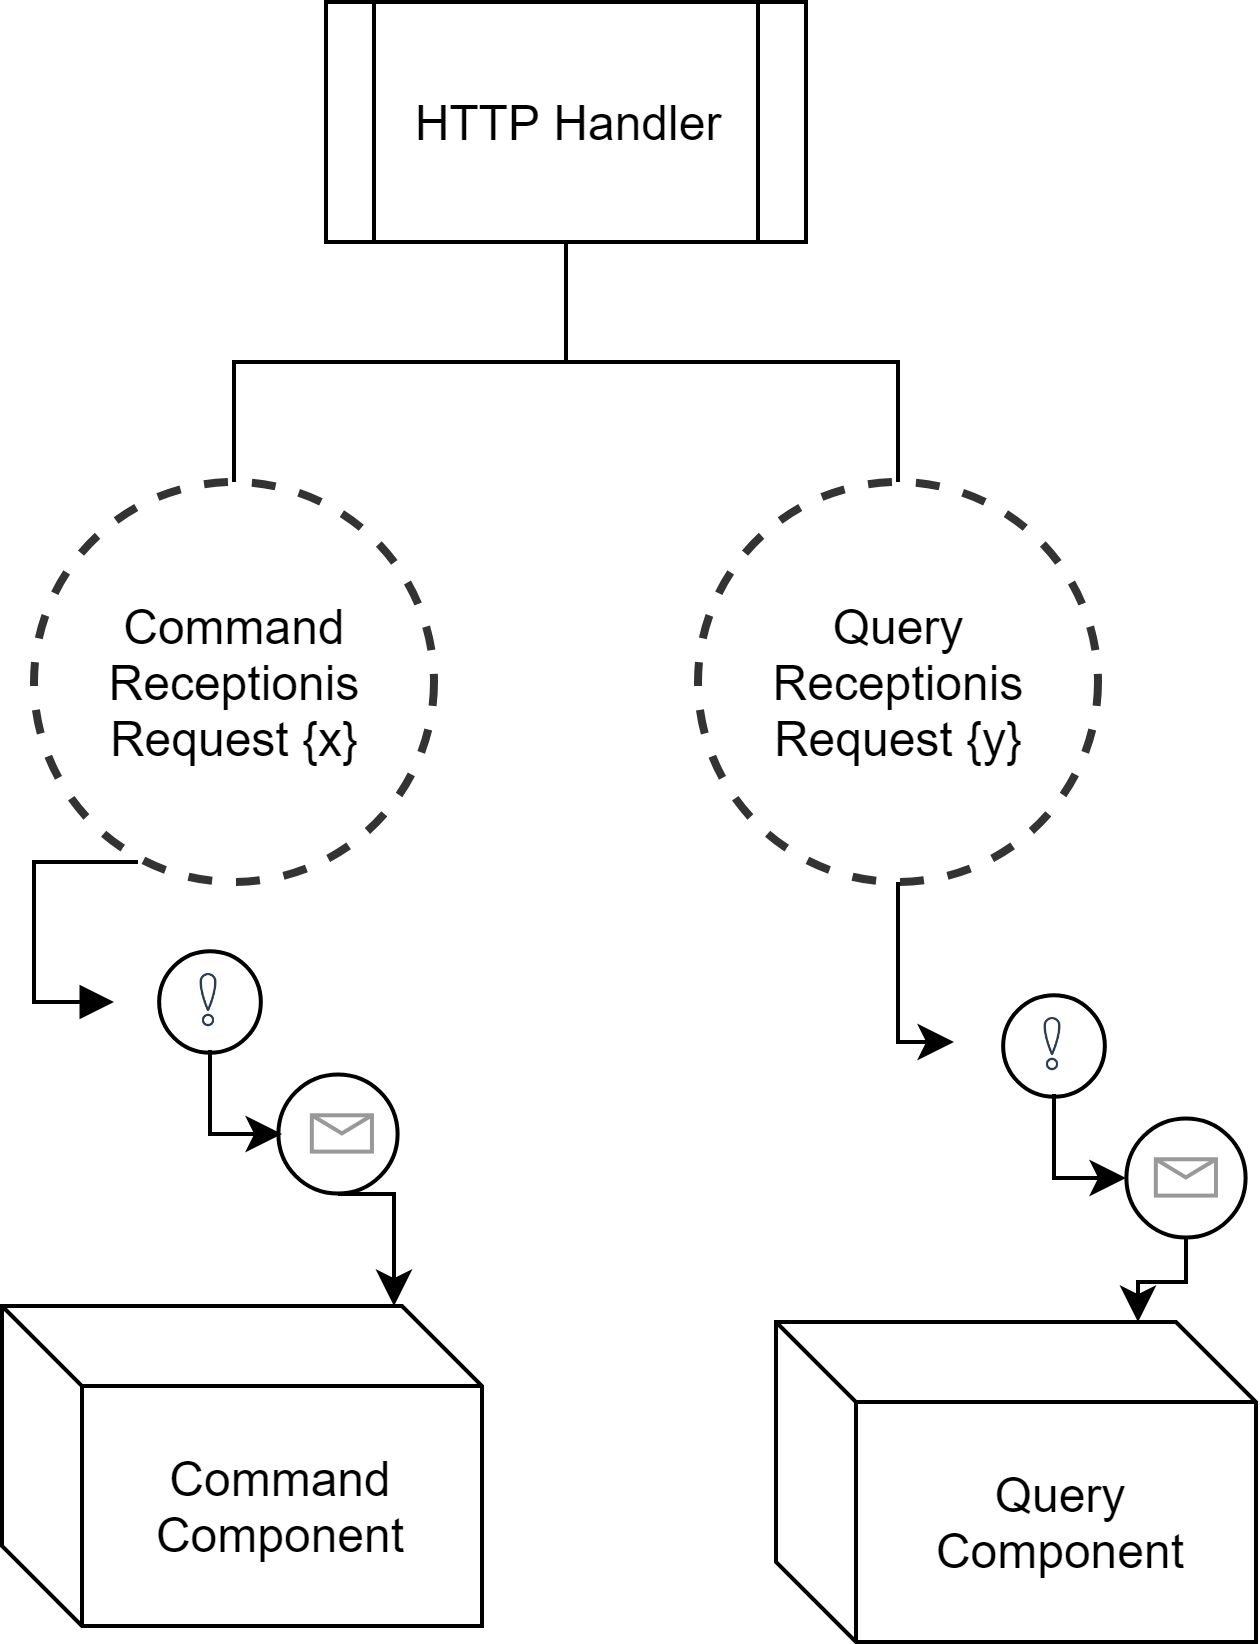
\includegraphics[width=0.5\linewidth]{gfx/implementation/apiActorModel}
    \caption{Actor Ansicht der API Komponente}
    \label{fig:implementation:apiActorModel}
\end{figure} 

\subsection{Query-Service}
Die Anwendung separiert wie bereits erwähnt Abfragen und Befehle nach dem \textit{CQRS}-Prinzip auf welches in Kapitel \ref{sub:transaction:cqrs} eingegangen wird. Die Abfrage Seite wird in der Implementierung der \textit{TyrolSky} Anwendung in einer eigenen Komponente realisiert. \\
Um eine Anfrage welche Daten des Systems abfragen möchte  abarbeiten zu können, überwacht die \textit{Query}-Komponente relevante Events welche im Event Sourcing aufgetreten sind, siehe dazu \ref{sec:implementation:eventSouring}. \\
Für jeden Typ von Abfrage wird dazu ein Ergebnis bereit gehalten, welches immer wieder aktualisiert wird. Wird ein relevantes Event im Event Sourcing gefunden, so wird das Ergebnis mit den neuen Eventdaten aktualisiert. Dadurch können bei eintreffenden Anfragen diese, durch das bereits vorbereitete Ergebnis, ohne weitere Abfragen an ein Datenbanksystem oder ähnliches, abgearbeitet werden. Jedoch sind die Resultate einer Abfrage nicht garantiert aktuell. Wird ein bereits eingetretendes Event zu spät in das vorbereitete Ergebnis miteingerechnet, bekommt der Anfragende das Ergebnis zurückgeliefert, welches vor dem Event gegolten hat. Deshalb wird diese Komponente nur für Anfragen von Benutzern verwendet und keine Entscheidungen innerhalb der Anwendung darauf aufgebaut.

\subsubsection{Aufbereitung von Resultaten}
\label{subsubsub:implementation:queryActorModel:resultPreparator}
Tretten neue Events auf, so wird die Resultatsliste aktualisiert. Wird eine neue Instanz der \textit{Query} Komponente gestartet, so muss diese zuerst alle im System befindlichen Events abarbeiten um ein aktuelles Ergebnis ausliefern zu können. Da dies bei einer vielzahl von Events Zeit und Ressourcen benötigt, werden aufbereitete Resultate selbst wieder abgespeichert. Dies passiert sporadisch nach einer bestimmten Menge an bearbeitenden Events. Wird das System neugestartet, kann auf das letzte abgespeicherte Resultat zurückgegriffen werden, und anschließend auf diesem weitergearbeitet werden. \\
Die Speicherung von Ergebnis führt jedoch zu Problemen wenn man die Verteilung der Komponente beachtet. Da jede Instanz seine eigenen Ergebnisse vorbereitet, müssen diese auch eigenständig gespeichert werden. Ansonsten ergeben sich beim Schreiben als auch beim Lesen konflikte zwischen den einzelnen Instanzen. Um dies zu umgehen wird entweder pro Instanz eine eigene permanente Persistierung, wie beispielsweise eine Datenbank, eingerichtet. Jedoch erhöht dies den Wartungsaufwand der Komponente da für jede Instanz eine eigene Datenbank gehalten werden muss. \\
Eine weitere Möglichkeit ist die Persistierung der Ergebnisse pro Komponente in einer globalen Datenbank. Wobei jeder Erzeuger von Ergebnissen seine Resultate mit einer Identifikation abspeichert. Dafür ist es jedoch erforderlich, dass Erzeuger von Ergebnissen eine eindeutige Identifikation besitzen. Dafür wurde ein globaler Namensservice implementiert, welcher im gesamten verteilten System eindeutige Namen vergibt. Meldet sich eine Komponenteninstanz vom System ab, werden alle Namen, welche an diese Instanz vergeben wurden, wieder freigegeben. Meldet sich eine Komponente wieder beim System an, so bekommt diese die wieder zuvor freigegebenen Identifikationen. Diese kann somit mit den Ergebnissen der vorherigen Komponente, welche sich nicht  mehr im System befindet, weiterarbeiten. Für die Umsetzung des globalen Namensservice wurde auf das Pattern \textit{Cluster Singelton}, welches in Abschnitt \ref{subsec:implementation:singeltons} erklärt wird, zurückgegriffen. \\
Durch die Verwendung einer globalen Datenbank, sowie auf daszurückgreifen eines globalen Namensservice ist während dem Betrieb der Anwendung der Wartungsaufwand auf ein minimum beschränkt. Weiters kann durch diese Variante sichergestellt werden, dass bei bei einem Neustart des Systems die Instanzen mit bereits zuvor erarbeiteten Resultaten weiterarbeiten können. 

\subsubsection{Implementierte Abfrage}
In der umgesetzten Implementierung werden in der \textit{Query}-Komponente Abfragen zur verfügung gestellt, welche dem Benutzer eine Übersicht über angebotente Flüge sowie den Status von Flugtickets geben. Insgesamt sind drei unterschiedliche Abfragen möglich:

\begin{enumerate}
    \item Status eines Flugtickets Abfragen
    \item Liste alle zur verfügung stehenden Flüge
    \item Passagierliste eines bestimmten Fluges
\end{enumerate}

Für die dritte Abfrage wurde jedoch eine andere Abfragevariante gewählt. Anstatt auf Events zu horchen, wird die Abfrage direkt an die entsprechenden Domaineninstanzen (siehe dazu Abschnitt \ref{subsec:implementation:domainService}) weitergegeben. Dies führt dazu, dass die Abfrage selbst länger dauert, da keine Ergebnisse vorgehalten werden. Jedoch ist die Abfrage selbst exakter da die Entitäten direkt abgefragt werden, und der Aufwand in der Entwicklung geringer. \\
Das Beispiel zeigt, dass je nach Anwendungsfall entschieden werden sollte wie die Abfrage von Daten exakt implementiert wird.

\begin{figure}
    \centering
    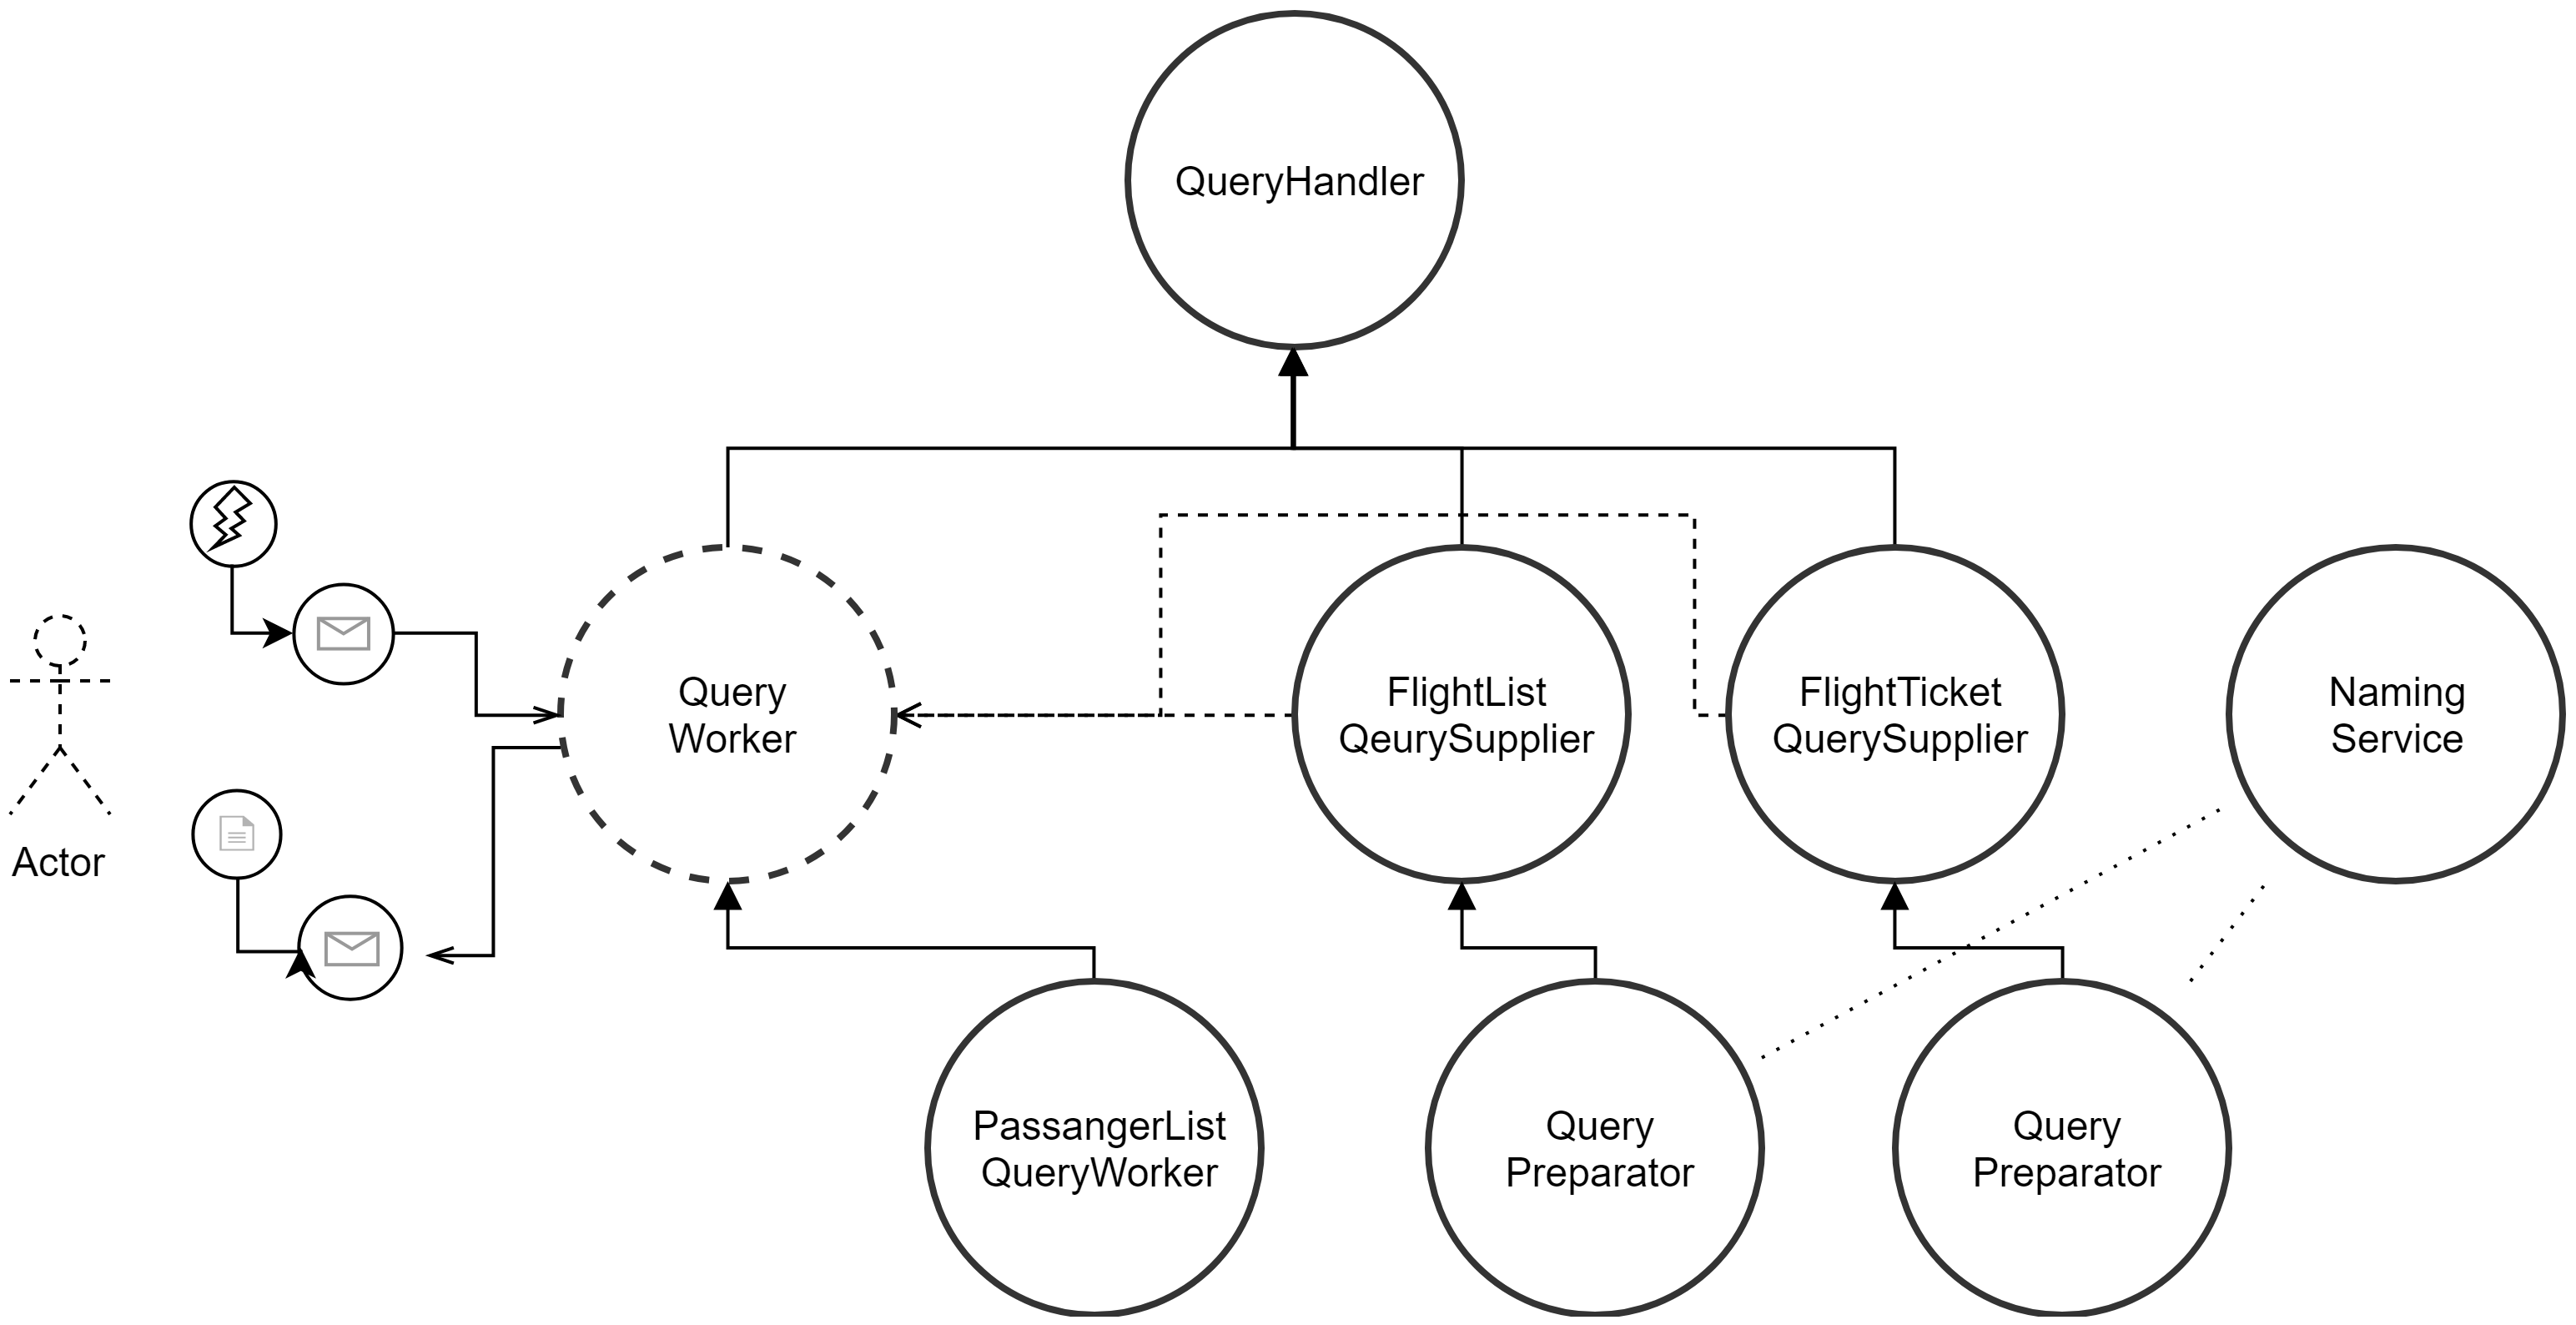
\includegraphics[width=\linewidth]{gfx/implementation/QueringServiceActorModel}
    \caption{Der Aufbau des Actor Systems der Query Komponente von \textit{TyrolSky}.}
    \label{fig:implementation:queryActorModel}
\end{figure} 

\subsubsection{Strukturierung}
Für die Abarbeitung einzelner Abfragen wird, ähnlich wie bei der Komponente \textit{API} aus Abschnitt \ref{subsec:implementation:apiComponente}, auch für die realisierung von Abfragen auf die Hilfe von kurzlebigen Actors gesetzt. Diese führen den eigentlichen Abfrageprozess durch, und verwenden dazu die entsprechenden Query-Actoren. In Abbildung \ref{fig:implementation:queryActorModel} ist der Aufbau der Query-Komponente in Form von Actors zu sehen. Darin ist zu erkennen, dass für jeden Typ von Abfrage ein Actor existiert welcher die Abfragen bearbeitet. 
Dieser Actor wird in der Implementierung als \textit{Supplier} bezeichnet und besitzt selbst wieder ein Child-Actor welcher sich um die Aufbereitung der Abfragedaten wie in Abschnitt \ref{subsubsub:implementation:queryActorModel:resultPreparator} beschrieben, kümmert. \\
Jede einzelne Abfrage beim \textit{Query-Service} wird einem neuem Worker-Actor zugewissen, welcher nur für den Zeitraum der Abfrage selbst instanziiert ist. Dieser fragt die benötigten Daten direkt vom, für die entsprechende Abfrage zuständigen, \textit{Supplier} ab. 

\subsection{Command-Service}
\label{subsec:implementation:commandService}
 Ähnlich wie beim \textit{Query-Service}, wird auch beim \textit{Command-Service} für jeden ankommenden Befehl ein eigener Actor gestartet, der für einen speziellen Typ von Anfrage zuständig ist. Für jeden Typ von Befehl innerhalb der Anwendung gibt es einen Actor welcher die Logik des Befehls beinhaltet. Jedoch werden in der Implementierung der einzelnen Kommandos meist neue Befehle an einen oder mehrere zuständige Actors aus dem Domain-Service erzeugt und weitergeleitet. \\
 In der vorliegenden Implementierung gibt es folgende unterschiedliche Typen von Kommandos, welche alle durch einen \textit{CommandHandler} repräsentiert werden:
 \begin{enumerate}
   \item Flüge erstellen
   \item Flug vorbereiten
   \item Ticket reservieren
   \item Ticket buchen
 \end{enumerate}
Die Abbildung \ref{fig:implementation:commandActorModel} zeigt den Aufbau des \textit{Command-Service}. Die Geschäftslogik ist in den Actors des \textit{Domain Serice} beherbergt. Somit ist die Tätigkeit der einzelnen \textit{CommandHandler} darauf begrenzt, die betroffenen Actors im \textit{Domain Serice} über die gewünschte Tätigkeit zu informieren und diese auszuführen. 
 \begin{figure}
  \centering
  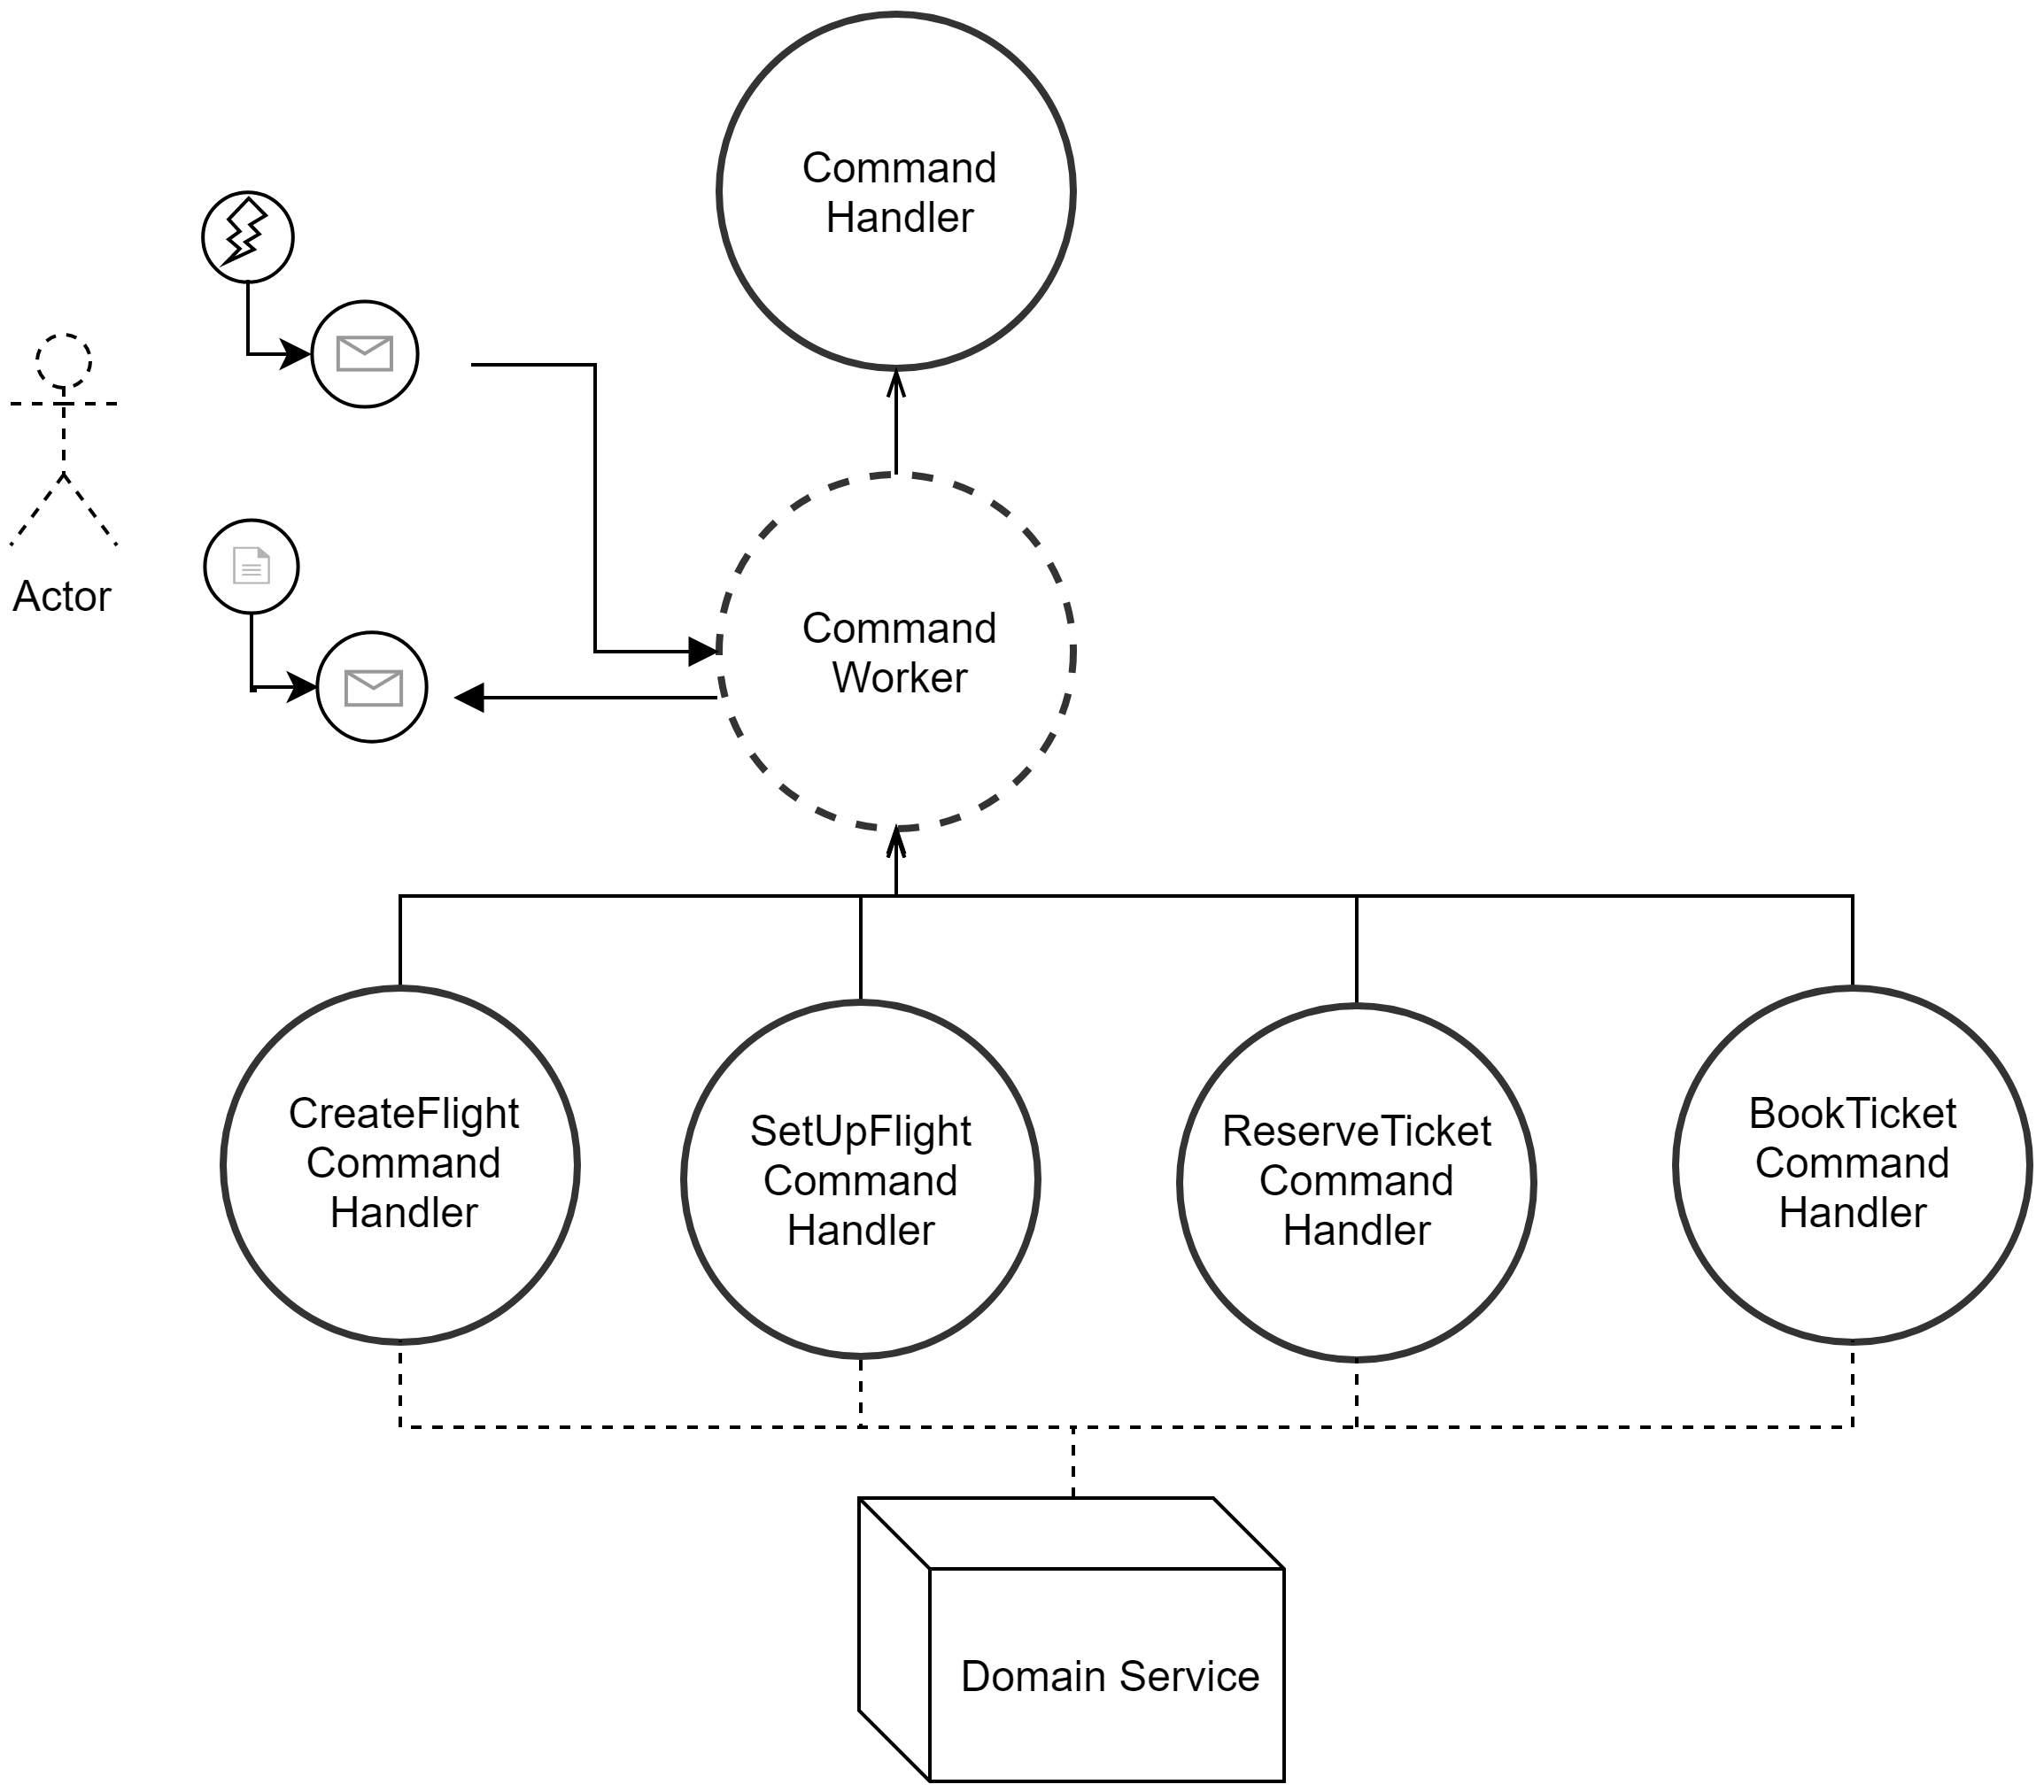
\includegraphics[width=0.8\linewidth]{gfx/implementation/CommandServiceActorModel}
  \caption{Der Aufbau des \textit{Command-Service} beinhaltet die Logik der einzelnen Befehle und leitete weitere Befehle an den \textit{Domain-Service} weiter }
  \label{fig:implementation:commandActorModel}
\end{figure} 



\subsection{Domain-Service}
\label{subsec:implementation:domainService} 
Die gesamte Geschäftslogik wie das verhalten von Flügen, Tickets und anderen Entitäten wird in der Komponente \textit{Domain-Service}  abgebildet. Die Actoren welche sich in dieser Komponente befinden, wurden so abgebildet das die Repräsentation der Anwendung selbst keine Rolle spielt. Das bedeutet, dass die Implementierung in dieser Komponente unabhängig davon umgesetzt wurde, ob die Anwendung selbst über das \textit{CQRS} Prinzip umgesetzt wird und ob die Interaktion mit dem Benutzer über eine \textit{HTTP} Schnittstelle umgesetzt wurde. \\
Die hier repräsentierten Entitäten, welche selbst ja wieder als Actoren repräsentiert werden, beinhalten neben der eigenen Logik auch einen Zustand welcher Persistiert wird. Dies wird durch \textit{Event Soucing} ermöglicht, welches in Abschnitt \ref{subsec:implementation:eventSouring} genauer beschrieben wird. Ereignisse welche in der Entität selbst auftretten, werden persistiert und bei einem späteren Neustart des dazugehörigen Actors wieder eingespielt. Mit diesem Prinzip sind alle nachfolgend beschriebenen Entitäten ausgestattet. \\
Um eine Verteilung der Entitäten zu ermöglichen werden diese in Form von \textit{Sharding} auf unterschiedliche Hosts verteilt. \textit{Sharding} selbst wird in Kapitel \ref{subsec:implementation:ApplicationDistribution} genauer betrachtet. Für eine Verteilung mittels \textit{Sharding} müssen Actoren bestimmt werden, welche anschließend verteilt werden. Alle Kindelement dieser Actoren werden anschließend an den gleichen Ort wie ihre Parents verschoben. Innerhalb des \textit{Domain Service} gibt es folgende Actoren welche Verteilt werden:
\begin{itemize}
    \item Flug Nummer (\textit{FlightNumber})
    \item Flug Ticket (\textit{FlightTicket})
    \item Buchungskoordinator (\textit{ChargingCoordinator})
\end{itemize}
Auf die genaue Aufgabe sowie die Implementierung dieser drei Actoren wird nun nachfolgend eingegangen.

\subsubsection{Flug Nummer}
Die Repräsentation der angebotenen Flüge selbst wird mit dem Actor \textit{FlightNumber} dargestellt. Dieser beinhaltet Informationen über Start- und Zielort und den Zeitraum an welchem der Flug zur verfügung steht. Für Informationen über einen Flug an einem bestimmten Datum wird ein neuer Actor herangezogen welcher den Operativen Flug darstellt. Der Actor \textit{OperateFlight} verwaltet Informationen über den Typ des Flugzeuges und die Passagierkapazität welche für diesen Flug angeboten wird. Informationen über Passagiere für diesen Flug werden jedoch nicht über den Actor selber verwaltet sondern an einen weiteren Actor, den \textit{FlightPassengerList} Actor welcher für diese Aufgabe spezialisiert ist, weitergereicht. \\
Der Actor \textit{FlightPassengerList} verwaltet für einen operativen Flug die verfügbaren Plätze. Dabei wird ihm. wie aus Abbildung \ref{fig:implementation:entityFlightNumber} zu entnehmen ist, von seinem \textit{Parent} dem \textit{OperateFlight} die verfügbare Kapazität, abhängig vom verwendeten Flugzeugtyp mitgeteilt. Der Actor verwaltet nun eine Liste mit reservierten sowie bereits gebuchten Ticket für diesen Flug. Die Tickets selbst werden jedoch wiederum in einem eigenen Actor repräsentiert. Dieser gehört jedoch nicht mehr in die Hierarchie der Flug Nummer sondern befindet sich in einer eigenen Verteilten Entität. \\
Nachrichten von ausserhalb dieser Hierarchie werden immer an den betreffenden \textit{FlightNumber} gesendet. Dieser leitetet die Nachricht weiter an den betroffenen \textit{OperateFlight} Actor, was nur möglich ist wenn die Nachricht auch die Informationen entsprechend bereitstellt. \\
Wird nun von einem \textit{CommandHandler} an den \textit{FlightNumber} Actor der Befehl gesendet ein Ticket zu reservieren, so wird dieser Befehl bis an die Passagierliste weitergereicht. Dort wird überprüft ob die Kapazitäten für eine neue Reservierung noch vorhanden sind. Ist dies der Fall, wird dieser Platz in der Passagierliste reserviert und ein neues Ticket erstellt. 
\begin{figure}
    \centering
    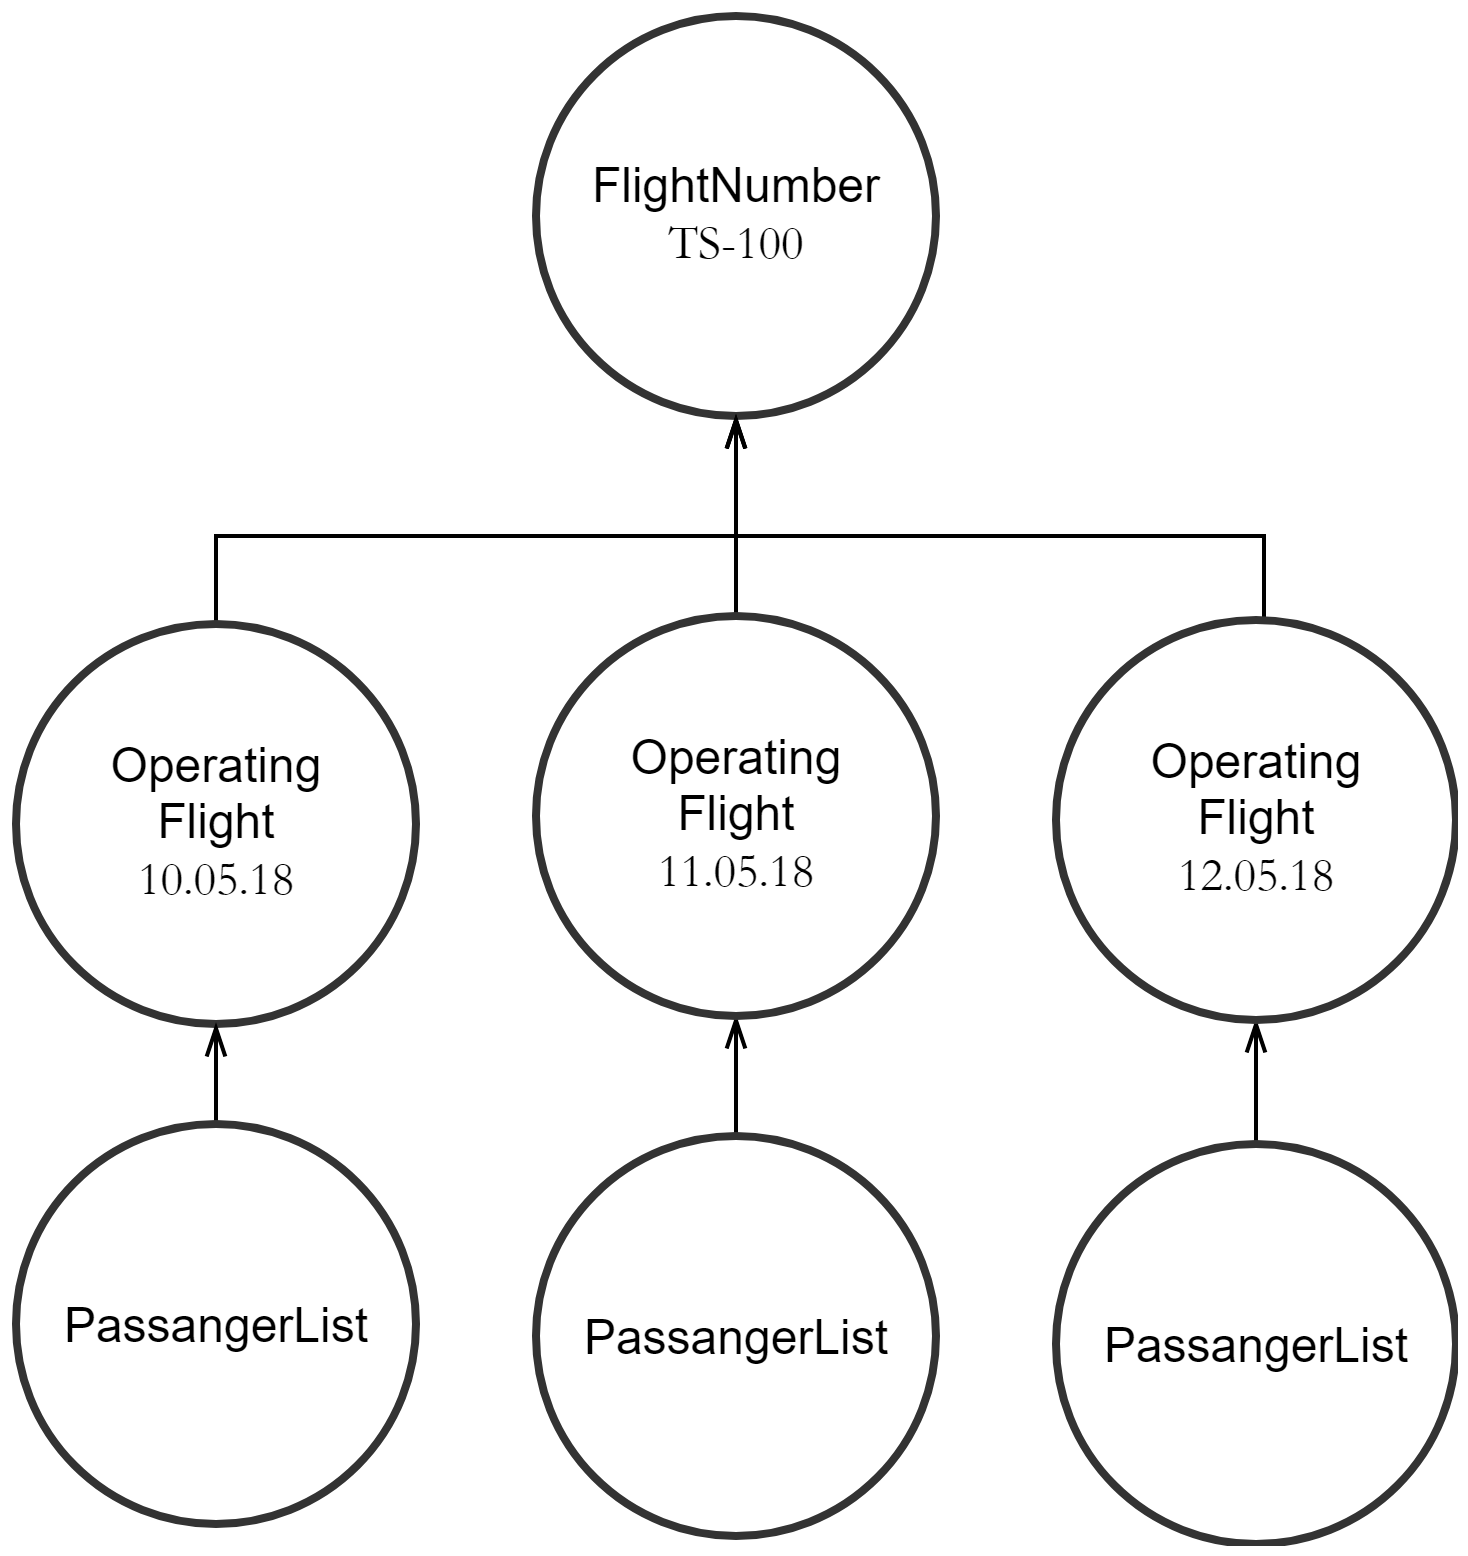
\includegraphics[width=0.65\linewidth]{gfx/implementation/FlightNumberSample}
    \caption{Darstellung eines Fluges welcher für drei Tage verfügbar ist.}
    \label{fig:implementation:entityFlightNumber}
\end{figure} 

\subsubsection{Flight Ticket}
Entscheidet ein \textit{PassangerList} Actor ein neues Ticket für einen Flug zu erstellen, so wird dieses Ticket als neue Entität im \textit{FlightTicket} Sharding erzeugt. \\
Die Entität selbst repräsentiert eine Ticketreservierung welche eine eindeutige Ticketidentifikation besitzt. Über diese Identifikation kann jedes Ticket exakt angesprochen werden. Ein Ticket repräsentiert neben dem Inhaber des Tickets auch der aktuelle Ticketstatus. Jedes Ticket kann sich in einem der folgenden Zustände befinden:
\begin{enumerate}
    \litem{Reserviert} Das Ticket wurde Reserviert und der Platz im Flugzeug ist bis auf weiteres durch dieses Ticket blockiert. Wird nach einer Konfigurierten Zeit kein Zustandswechsel vollzogen, so storniert sich das Ticket selbstständig und der Platz wird wieder freigegeben.
    \litem{Gebucht} Der Bezahlvorgang für dieses Ticket konnte erfolgreich abgeschlossen werden und der gebuchte Sitzplatz bleibt ohne Zeitablauf für dieses Ticket reserviert.
    \litem{Stoniert} Das Ticket wurde entweder vom Benutzer selbst storniert. Weiters ist es möglich das der Bezahlvorgang nicht erfolgeich durchgeführt werden konnte oder das Ticket durch ablaufen eines Zeitfensters selbst storniert hat. Der reservierte Platz steht wieder für neue Reservierungen zur verfügung
    \litem{Bezahlvorgang läuft} Wird ein Ticket gebucht so wird dadurch der Bezahlvorgang gestartet. Während dieser läuft befindet sich die Reservierung in diesem Status. Verläuft der Bezahlvorgang erfolgreich wird das Ticket in den Status \textit{Gebucht} wechseln ansonsten in den Status \textit{Stoniert}.
\end{enumerate}
Für die Implementierung eines Zeitfensters für den Abblauf eines Tickets wird bei der reservierung des Tickets eine Nachricht geplant. Das bedeutet es wird zu beginn der reservierung vom Ticket selbst eine Nachricht an sich selbst versendet welche signalisiert das eine Zeitfenster abgelaufen ist. Jedoch wird dabei beim versenden mittels dem \textit{Akka.Net} Framework eine Zustellzeit angegeben. Wird die Nachricht zugestellt, kann der Actor selber entscheiden ob sie noch relevant ist. Ist beispielsweiße das Ticket mittlerweile in einem Zustand in welchem eine Stornierung nicht mehr notwendig ist, kann die Nachricht verworfen werden, ansonsten kann die Stornierung der Reservation gestartet werden. \\
Der Bezahlprozess für die Buchung eines Tickets wird einem Koordinator übergeben welche die Buchung selbst steuert. Der \textit{FlightTicket} Actor erhält von diesem Koordinator nach dem Bezahlvorgang eine Nachricht über den ausgang des Vorgangs und ändert anschließend den Zustand des Tickets entsprechend. 

\subsubsection{Buchungskoordinator}
\label{subsub:implementation:ChargingCoordinator}
Wird ein bereits reserviertes Ticket gebucht, so erzeugt das Ticket für den Bezahlvorgang einen neuen Buchungskoordinator. Dieser Buchungskoordinator bekommt eine eigene Buchungs Identifikation vom Ticket zugewissen. Der Buchungskoordinator selbst wird wie auch die zuvor beschriebenen Entitäten über \textit{Sharding} verteilt. Somit kann ein Ticket und der dazugehörige Buchungskoordinator an einem unterschiedlichen Host instanziiert werden. \\
Die Aufgabe des Buchungskoordinator ist es, den gewünschten Betrag von einer externen Bankenschnittstelle abzubuchen. Die Bankenschnittstelle selbst wurde für die Umsetzung dieses praktischen Beispieles simuliert und ist in Kapitel \ref{subsec:implementation:bankApi} näher beschrieben. Ein austausch von transaktionallen Informationen über eine externe Schnittstelle ist jedoch durch verschiedene Faktoren problematisch. Um die Konsistenz von Abbuchungen und Ticketstatus zu gewährleisten, darf es nicht dazu kommen das Informationen bei der Übertragung verloren gehen. Wie jedoch in Kapitel \ref{sec:distributedSystems:wrongAssumptions} bereits besprochen, kann ein Datenaustausch über ein Netzwerk immer Fehlschlagen. Deshalb prüft der Buchungskoordinator solange den Status einer Anfrage zum Bankensystem, bis von diesem eine nicht änderbares Buchungsresultat gesendet wird. \\
Wird ein Buchungskoordinator erstellt, so werden folgende Schritte ausgeführt:
\begin{enumerate}
    \item Bezahlprozess bei Bank starten
    \item Prüfen ob Bezahlvorgang bei der Bank abgeschlossen
    \item Vorgang \textit{2.} solange wiederholen bis unveränderlichbares Ergebnis von der Bank empfangen wird.
    \item Ersteller des Bezahlprozess mit Ergebnis der Bezahlung Informieren
\end{enumerate}
Durch den Umstand, das auch ein der \textit{ChargingCoordinator} mittels \textit{Event Sourcing} seinen zustand persistiert, kann auch nach einem Ausfall des Systems am Abbuchungsprozess weitergearbeitet werden sobald das System wieder startet. \\
In Abbildung \ref{fig:implementation:ChargingCoordinatorSample} ist der Aufbau des \textit{ChargingCoordinators} abgebildet. Dabei ist zu erkennen das der Koordinator selbst keine weiteren \textit{Childs} mehr besitzt. Stattdessen wird für die eigentliche Abfrage an die Bankenschnittstelle ein anderer Actor verwendet, welche sich nicht unter ihm befindet. Dieser nimmt somit nicht am \text{Sharding} teil und ist fix an jedem Host verfügbar, worauf in Abschnitt \ref{sec:implementation:externalApi} noch genauer eingegangen wird. Dadurch wird bei einer neuverteileing der \textit{Shards}, siehe dazu Abschnitt \ref{subsec:implementation:ApplicationDistribution}, eine bestehende Verbindung zur Bank nicht abgebrochen. 
\begin{figure}
    \centering
    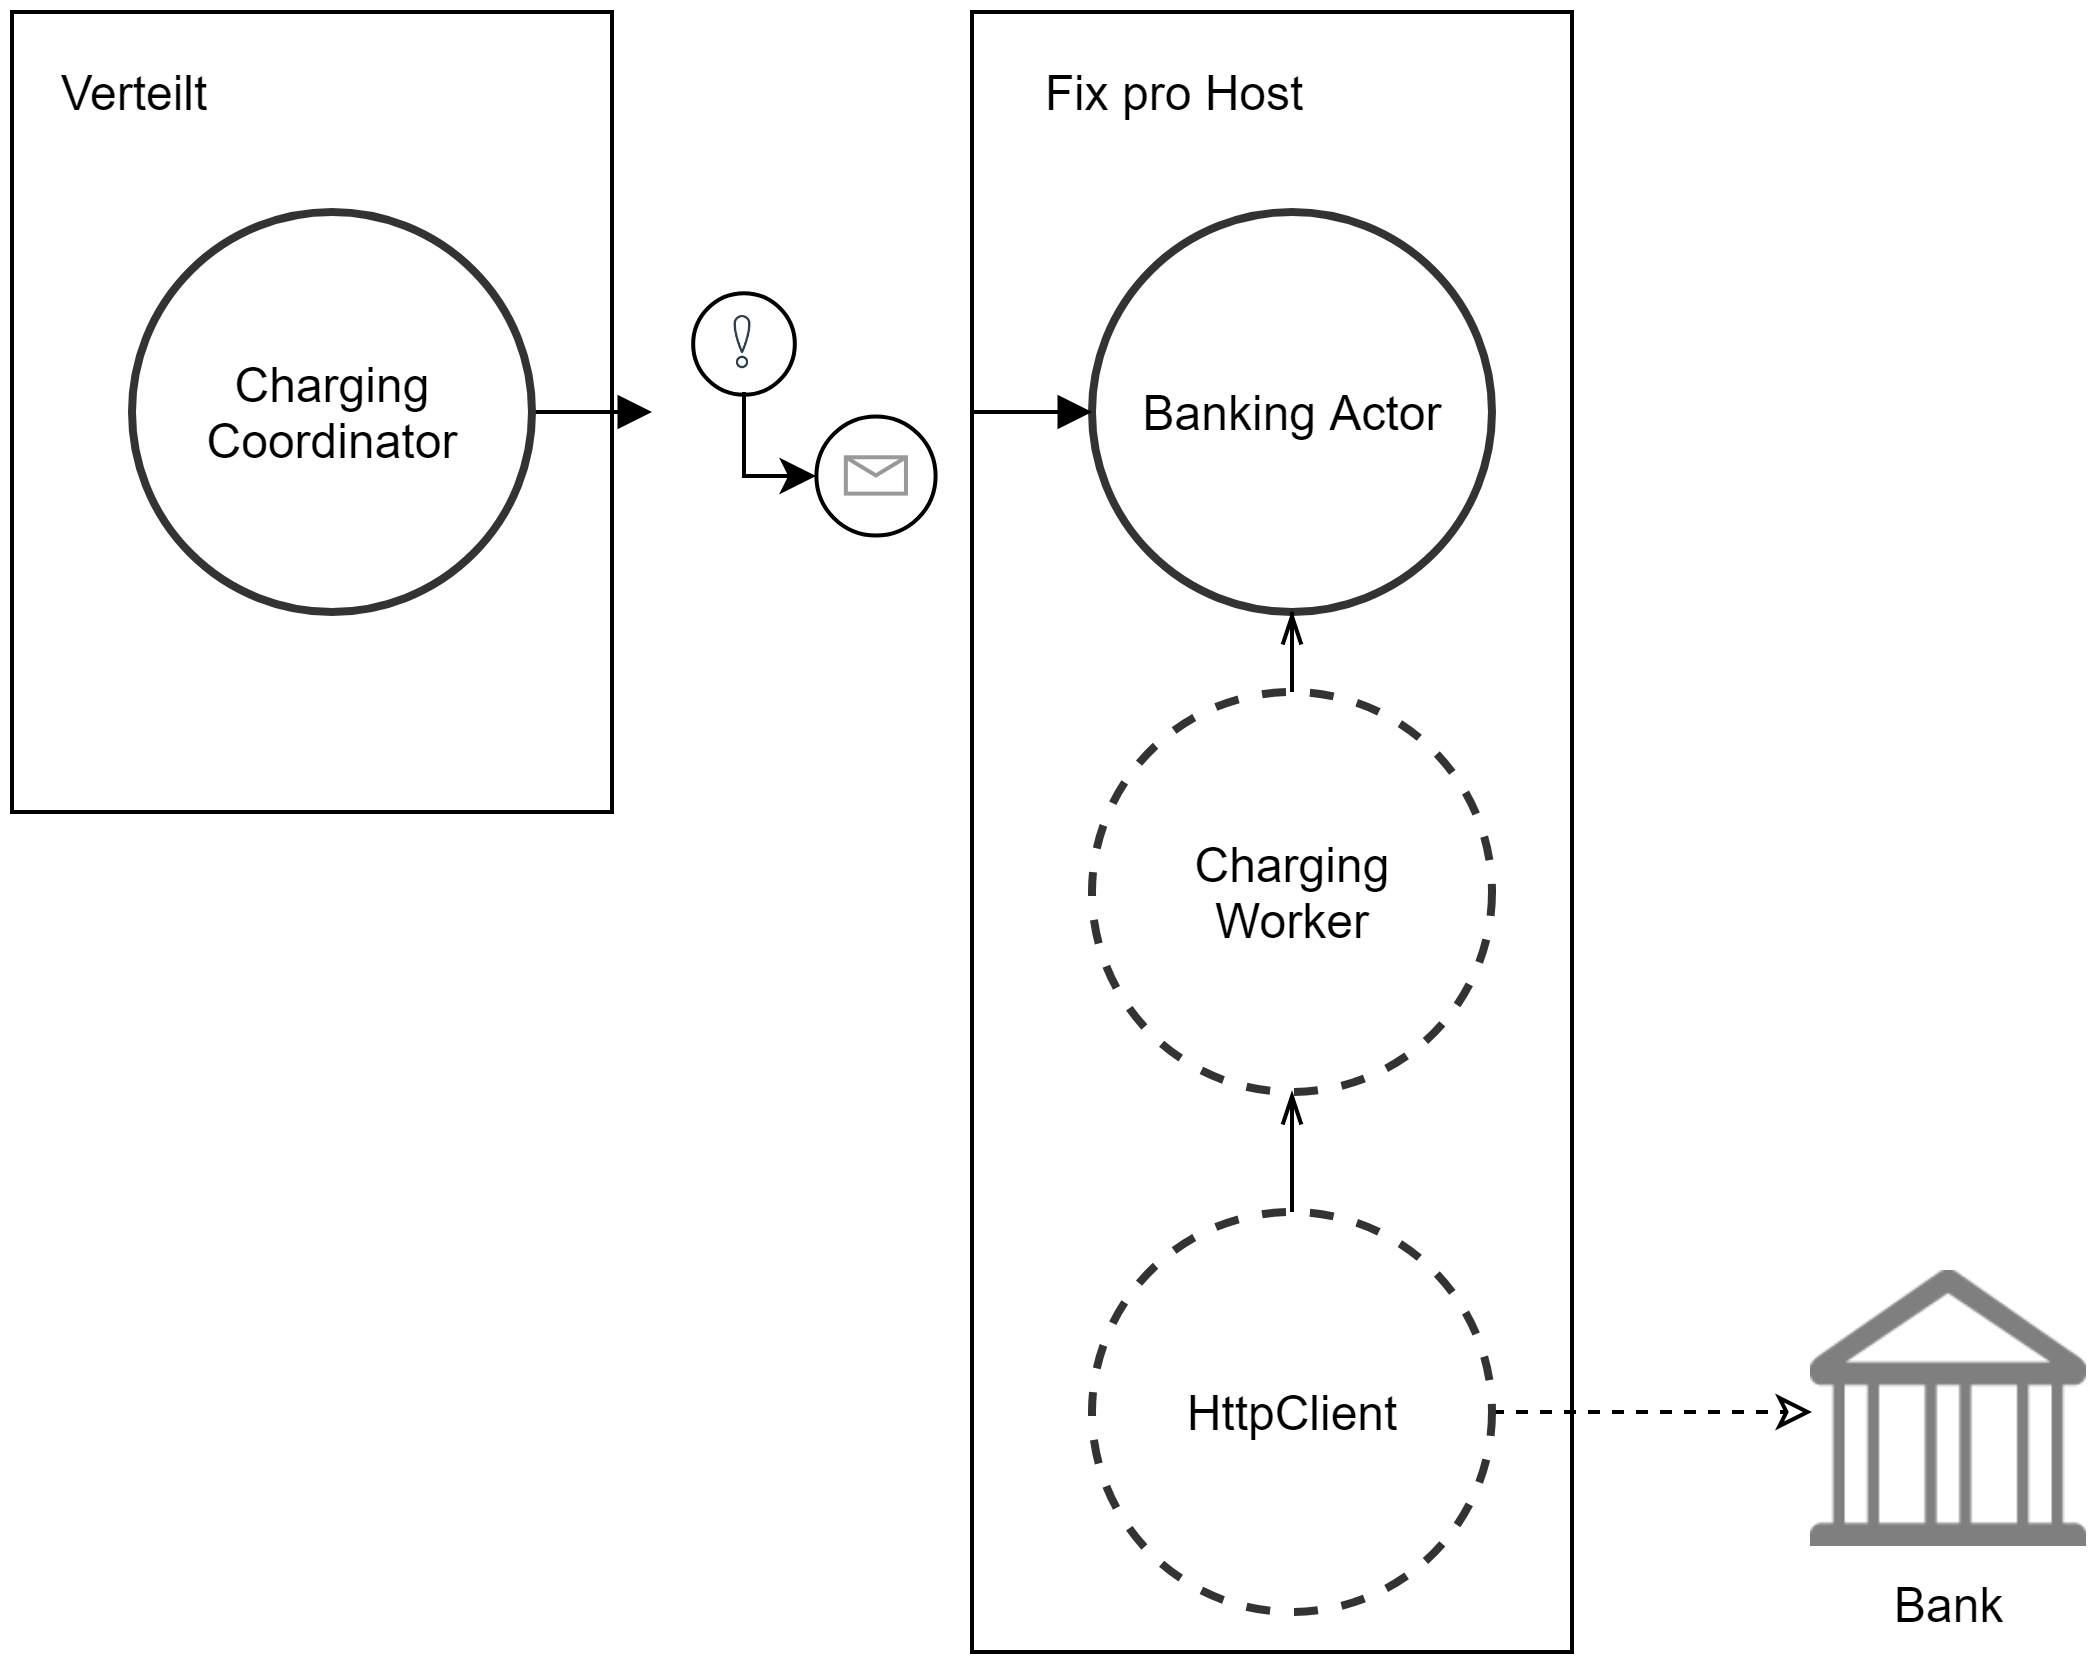
\includegraphics[width=0.65\linewidth]{gfx/implementation/ChargingCoordinatorSample}
    \caption{Modelierung des verteilten Buchungskoordinator, welcher eine nicht verteilten Actor für Anfragen an Banken verwendet}
    \label{fig:implementation:ChargingCoordinatorSample}
\end{figure}




\section{Implementierung von Event Sourcing}
\label{sec:implementation:eventSouring}
Die Persistierung der Daten basiert auf dem \textit{Event Sourcing}, wie in Abschnitt \ref{sec:eventSourcing} beschrieben wird. Das Prinzip von \textit{Event Sourcing} ist es, aufgetretene Ereignisse abzuspeichern und gegebenenfalls wieder einzuspielen, um so einen Zustand reproduzieren und nachvollziehen zu können \citep{betts2013CQRSEventSourcing}. \\
Das verwendete Framework \textit{Akka.net} bietet eine grundlegende Unterstützung für \textit{Event Sourcing} \citep{Akka.netCommunityAkka.NETDocumentation}. Dabei werden Events als Nachrichten repräsentiert, welche dem Framework übergeben und anschließend abgespeichert werden. 
Erst nach erfolgreicher Speicherung des Events, kann auf das Event selber reagiert werden. Dadurch wird verhindert das Aktionen zu Events ausgeführt werden, jedoch das Event nicht persistiert werden kann. Weiters bietet \textit{Akka.Net} die Möglichkeit, Events zu einem späteren Zeitpunkt wieder einzuspielen und mit einer anderen Verhalten darauf zu reagieren als beim vorherigen Auftreten des Events. Dies ist erforderlich, damit Ereignisse welche in der Vergangenheit aufgetreten sind,  wieder eingespielt werden können. Dabei wird die Einspielung eines Events meist nicht gleicht behandelt, als wie wenn das Ereignisse gerade aufgetreten ist. Wird beispielsweise bei einer Ticketbuchung das Bankkonto belastet, und wird die Buchung nachträglich wieder eingespielt, sollte zwar der Status des Tickets aktualisiert werden, eine neuerliche Kontobelastung ist aber nicht mehr erforderlich. Deshalb werden in diesem Beispiel zwei Verhalten für das gleiche Ereignis benötigt.
\subsection{Aggregate Root}
Um die Implementierung der einzelnen Entitäten zu vereinfachen, wurde die Logik für \textit{Event Sourcing} in einer Basisklasse zusammengeführt, von welcher die eigentlichen Entitäts-Actoren ableiten. 
Die eigentliche Logik für die Speicherung des Events übernimmt die Methode \textit{Emit(IDomainEvent e, Action a)} die in derBasisklasse des Entitäts-Actors verfügbar ist. Der Verwender der Methode \textit{Emit()} übergibt dieser ein Event, welche alle Informationen über das aufgetretene Ereignis enthält. Weiters wird eine Action übergeben die ausgeführt wird, sobald das Event erfolgreich im \textit{Event Store} abgelegt wurde. Während der Speicherung des Events wird von \textit{Akka.net} sichergestellt, dass keine weiteren Nachrichten vom Actor abgearbeitet werden. Die Methode \textit{Emit()} speichert nicht nur das Event im \textit{Event Store} ab sondern ändert den Zustand des Actors und führt die übergebene Action aus. Dafür wird, nach der Speicherung des Events, die übergebene Action ausführt und die abstrakte Methode \textit{UpdateState()} aufgerufen. \\
Jede Ausprägung der abstrakten \textit{Aggregate Root} Klasse muss die Methode \textit{UpdateState(IDomainEvent e)} implementieren. Diese wird direkt nach der erfolgreichen Persistierung des Events von der Methode \textit{Emit()} aufgerufen. Die Implementierung der Methode \textit{UpdateState()} sollte den Zustand des Actors, entsprechend dem aufgetretenen Event, verändern. Im Gegensatz zu der zuvor übergebenen \textit{Action}, wird \textit{UpdateState()} auch bei einer historischen Einspielung der Events aufgerufen. Die Methode \textit{UpdateState()} soll mit allen unterschiedlichen Event Varianten, welche innerhalb des Actors auftreten, umgehen können und dementsprechend die interne Repräsentation des Actors verändern. Änderungen des internen Zustands des Actors, außerhalb der Methode \textit{UpdateState()}, führen bei einer Wiedereinspielung der Ereignisse zu unterschiedlichen Zuständen des Actors . Deshalb sollen sämtliche Änderungen des Zustands des Actors innerhalb der Methode \textit{UpdateState()} ausgeführt werden. \\
Nach dem Aktualisieren des Actors-State prüft die Methode ob ein \textit{Snapshot} ausgeführt werden soll, mehr dazu in Abschnitt \ref{subsec:implementation:eventSouring:Snapshot}. Abschließend wird die zuvor übergebene Methode \textit{Action} aufgerufen, welche die eigentliche Logik enthält, wie auf das aufgetretene Ereignis reagiert werden kann. Hier können andere Actors über das aufgetretene Ereignis benachrichtigt werden. Die Action wird nur aufgerufen, wenn das Event tatsächlich Auftritt, bei einer Wiedereinspielung des Events wird ausschließlich die Methode \textit{UpdateState} aufgerufen. \\ 

In der Abbildung \ref{fig:implementation:eventSourcingAggregateRoot} ist der beschriebene Prozess schematisch abgebildet. Darauf ist auch zu ersichtlich, dass zwei unterschiedliche Datenbanken verwendet werden, um Snapshots und Events abzubilden.
\begin{figure}
    \centering
    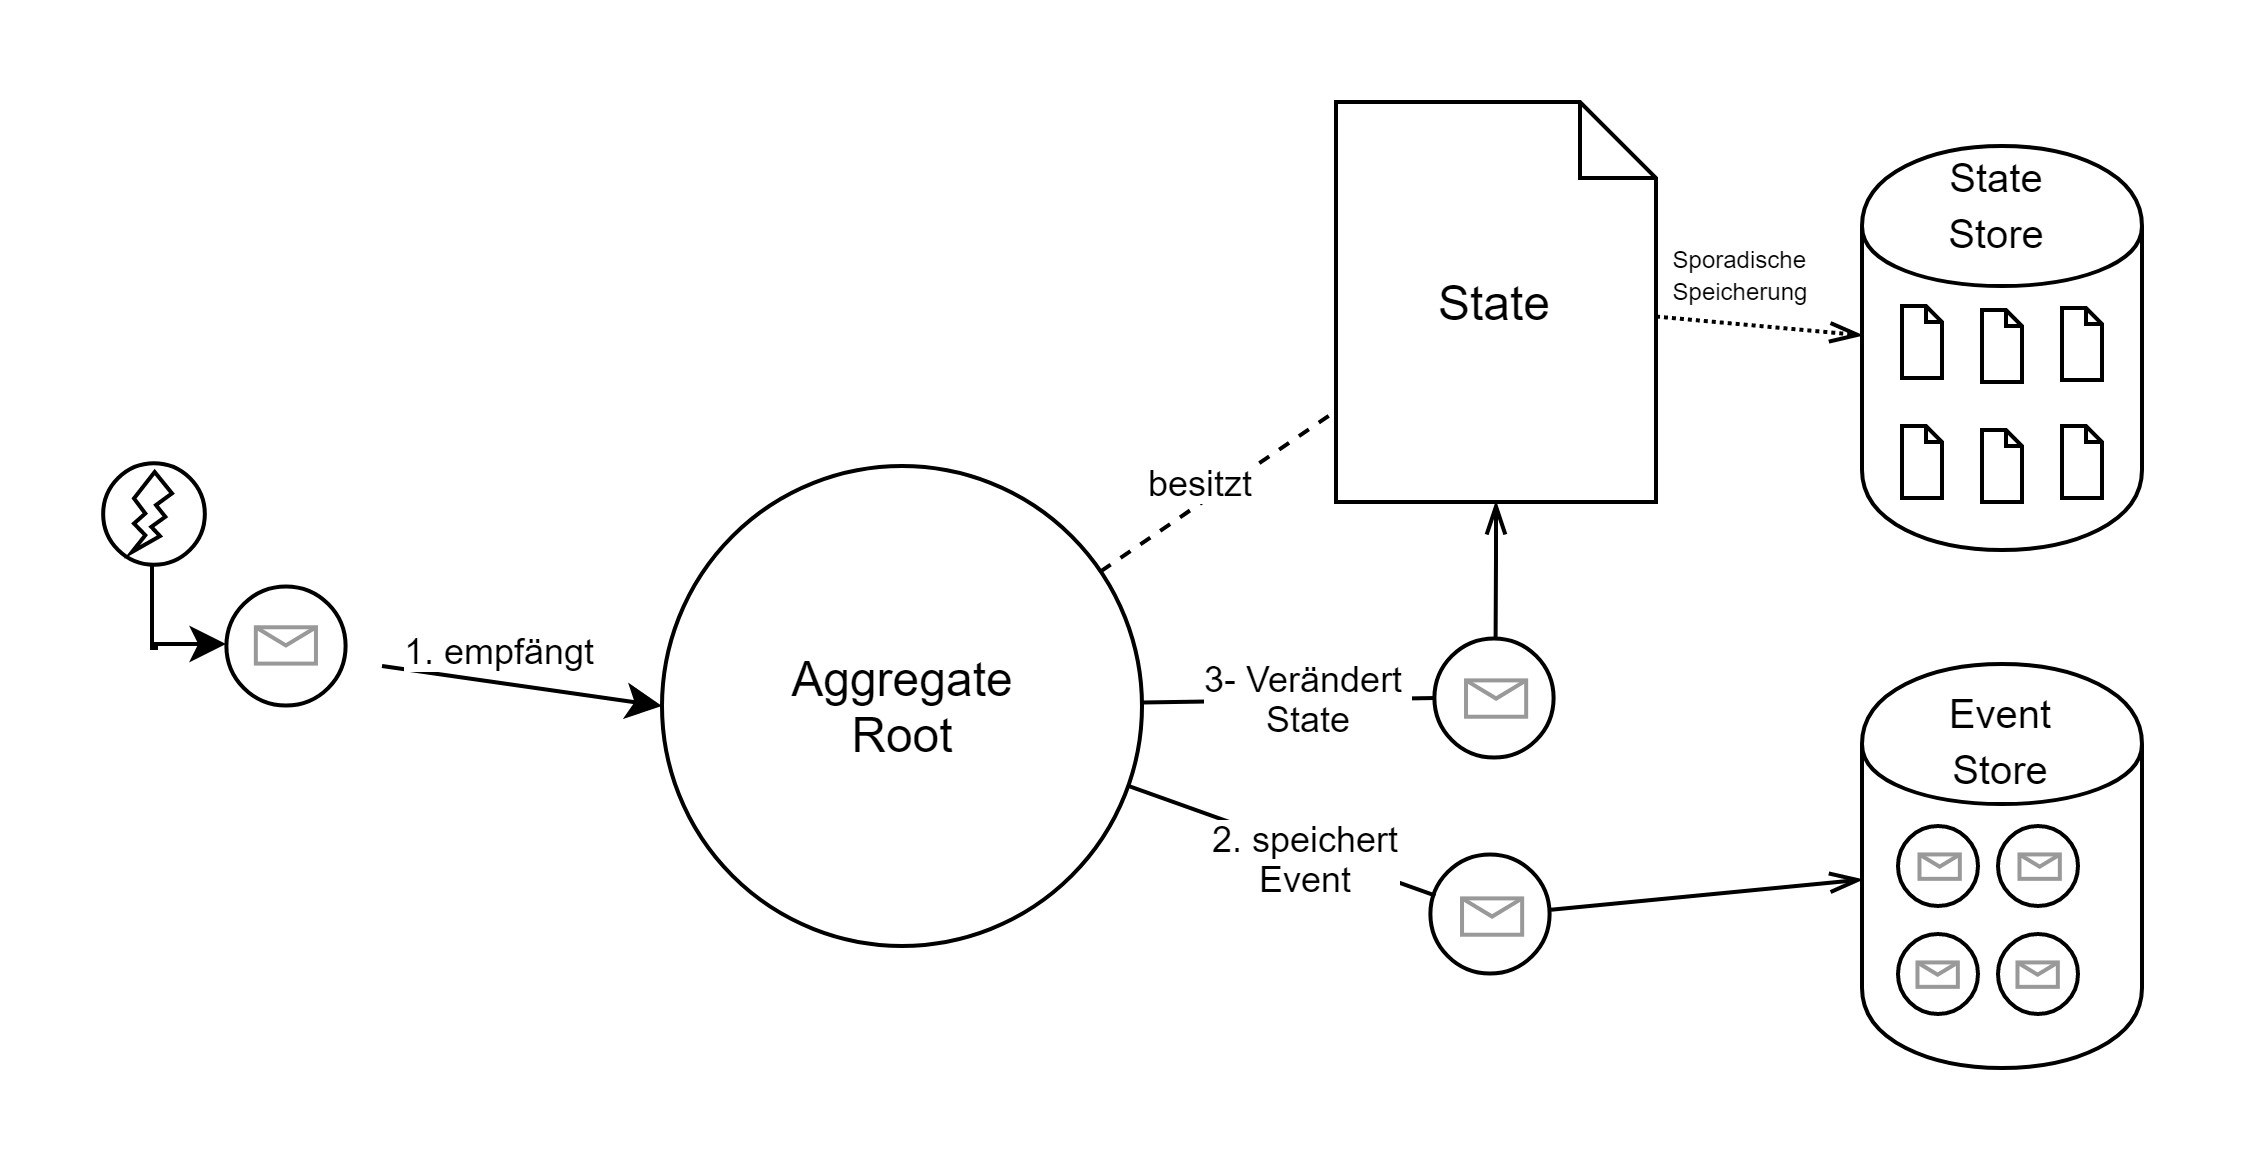
\includegraphics[width=\linewidth]{gfx/implementation/EventSourcingAkka}
    \caption{Ablauf der Speicherung eines Events innerhalb eines \textit{Aggregate Root} Actors mit \textit{Event Sourcing} und \textit{Snapshots}.}
    \label{fig:implementation:eventSourcingAggregateRoot}
\end{figure} 

\subsection{Snapshot}
\label{subsec:implementation:eventSouring:Snapshot}
Um bei einer Wiedereinspielung der Ereignisse für einen Actor nicht alle bereits aufgetretenen Ereignisse  wieder einspielen und dabei für jedes Ereignis die Methode \textit{UpdateState()} aufrufen zu müssen, wird regelmäßig ein Abbild des aktuellen Actorzustands gespeichert. Dies passiert innerhalb der Methode \textit{Emit()}. In der vorliegenden Implementierung wird nach jedem zwanzigsten Event ein Snapshot erstellt. Dafür wird die interne Datenrepräsentation eines Actors in eine eigene serialisierbare Klasse, den \textit{Actor State}, abgebildet. Diese Klasse wird auch bei der oben besprochenen Methode \textit{UpdateState()} verändert. Wird nun ein Snapshot erstellt, so wird der aktuelle \textit{Actor State} in einer dafür vorgesehenen Datenbank abgespeichert. Zusätzlich zum aktuellen \textit{State} wird die Sequenznummer des letzten Events, welches zu diesem \textit{State} geführt hat, gespeichert. Während der Erstellung des Snapshots kann der Actor selbst jedoch weiterhin Nachrichten abarbeiten. Dies beeinträchtigt nicht die Konsistenz der Datenrepräsentation. Durch die Zuordnung von einer Sequenznummer zu einem abgespeicherten \textit{State} werden Events, welche während der Erstellung des Snapshots anfallen, nicht mehr zum Snapshot dazu gezählt und somit später wieder auf Basis des vorhandenen Snapshots eingespielt. \\
Wird nun ein gestoppter Actor, dessen Zustand mittels \textit{Event Sourcing} persistiert wurde, wieder gestartet, so kommt es zur Wiederherstellung des vorherige Zustand. Während vergangene Ereignisse eingespielt werden, kann der Actor keine neuen Nachrichten verarbeiten. Diese verbleiben solange in der Mailbox des Actors bis die Einspielung abgeschlossen ist. \\
Die Wiederherstellung eines Actors wird erreicht, in dem zuerst der zuletzt verfügbare \textit{Snapshot} für den Actor in der Datenbank gesucht wird. Anschließend wird der Zustand des entsprechenden \textit{Snapshots} dem Actor als \textit{State} zugeteilt. Nun werden alle Events, welche nach der Erstellung des Snapshots angefallen sind, in der zeitlichen Reihenfolge ihres Auftretens wieder in den Actor eingespielt. Nach dem letzten eingespielten Event ist der Zustand des Actors exakt der gleiche wie vor dem Stoppen des Actors. \\
Wie bereits angedeutet, wird nicht von allen Actors innerhalb der \textit{TyrolSky}-Anwendung mittels \textit{Event Sourcing} der aktuelle Zustand gespeichert. Nur Actors, welche einen für die Konsistenz der Anwendung notwendigen Zustand repräsentieren, wurden mit \textit{Event Sourcing} persistiert. Dies sind folgende Actors: 
\begin{itemize}
    \item{\textit{OperateFlight}}
    \item{\textit{FlightPassangerList}}
    \item{\textit{ChargingCoordinator}}
    \item{\textit{FlightTicket}}
    \item{\textit{FlightNumber}}
    \item{\textit{DistributedUniqueNamingService}}
\end{itemize}
Die ersten fünft genannten Actors sind Teil der Komponente \textit{Domain Service} und präsentieren die Domäne der \textit{TyrolSky}. Der verbleibende Actor \textit{DistributedUniqueNamingService} dient zur Implementierung der unterschiedlichen \textit{Query}-Aufbereiter des \textit{Query-Services}, welche bereits in Abschnitt \ref{subsubsub:implementation:queryActorModel:resultPreparator} beschrieben wurden.

\subsection{Version Problematik}
Es muss sichergestellt werden, dass Events bei einer späteren Wiedereinspielung gleich behandelt werden als zu dem Zeitpunk, an welchem das Ereignis tatsächlich aufgetreten ist. Ändert sich die Implementierung für einen bestimmten Event-Typ innerhalb der Methode \textit{UpdateState()}, welche auch vergangene Events verarbeitet, kann es zu Inkonsistenzen der Anwendung kommen. Deshalb muss bei einer Anpassung von dem vorhandenem Code der \textit{UpdateState()} Methode entschieden werden, ob dies Codeänderung auch für ältere Events zulässig ist. Wird durch die Codeanpassung ein anderer Actor State als zuvor berechnet, kann nicht mehr der Originalzustand zum Zeitpunk des Ereignisses herbeigeführt werden. \\
Soll ein neues Verhalten für ein bereits vorhandenes Ereignis benötigt werden, wird ein neuer Event-Typ eingeführt. Durch die Versionierung von Event-Typen können keine Inkonsistenzen durch Codeänderungen in das System gebracht werden. 


\section{Verteilung der Anwendung}
\label{subsec:implementation:ApplicationDistribution}
Eine wesentliche Anforderung an die Praxisanwendung ist, dem Anforderungskatalog unter Kapitel \ref{sec:Eruierung:technicalRequierements} entsprechend, die Fokussierung der Softwarearchitektur auf die auf Verteilung der gesamten Anwendung. Dies kann erreicht werden, indem die Anwendung in verschiedene Services unterteilt wird, siehe dazu in Abschnitt \ref{sec:implementation:serviceAndComponentOrientation}. \\
Für die Erstellung von Instanzen dieser Komponenten wurden vier verschiedene Konsolenanwendungen implementiert, wobei für jeden Service ein eigene Anwendung geschrieben wurde. Eine Ausnahme stellen hier \textit{Domain-Service} und \textit{Command-Service} dar, denn sie operieren in einer gemeinsamen Anwendung. \\
Die Verbindung zwischen den einzelnen Komponenten wird mit der Cluster-Unterstützung umgesetzt, welche \textit{Akka.net} mitliefert und im nachfolgenden Abschnitt \ref{subsec:implementation:akka:cluster} beschrieben ist. 

\subsection{Cluster}
\label{subsec:implementation:akka:cluster}
Die Cluster-Funktionalität von \textit{Akka.net} bietet die Möglichkeit, zusammengehörende Anwendungen über ein Netzwerk zu verbinden und somit einen Cluster zu formen. Für den Benutzer der Anwendung harmoniert der Cluster als eine geschlossene Einheit. Dazu werden mittels einem \textit{Peer-to-Peer} Netzwerk alle teilnehmenden Anwendungen untereinander verbunden. Über ein Protokoll, das sogenannte \textit{Gossip}, genauer beschrieben in Abschnitt \ref{subsec:implementation:gossip}, werden Informationen zum Zustand des Clusters ausgetauscht. Jede am Cluster teilnehmende Anwendung wird als Node bezeichnet. Somit bilden zwei oder mehr Nodes einen Cluster \citep{akkaInAction}. \\
Jede Anwendung bekommt Rollen zugewissen, welche es zur Laufzeit übernehmen kann. Eine Rolle definiert in \textit{Akka.net} ein Aufgabengebiet innerhalb des Clusters. Für \textit{TyrolSky} wurden die fünf, in Abschnitt \ref{sec:implementation:serviceAndComponentOrientation}definierten, Services als Rollen herangenommen. Tritt eine Anwendung dem Cluster bei, so gibt sie während dem Eintrittverfahren bekannt, welche Rollen sie im Cluster übernehmen kann. Eine Rolle kann somit mehrfach im Cluster vorhanden und mehrfach redundant ausgelegt sein. \\
Die Kommunikation zwischen den Komponenten erfolgt innerhalb des \textit{Akka.net} Cluster entweder über Routing-Mechanismen, siehe Abschnitt \ref{subsec:implementation:akkaRouting}, oder über verteilte Daten, welche in \textit{Shards} organisiert sind, nachzulesen in Abschnitt \ref{subsec:implementation:akkaSharding}. 

\subsection{Routing}
\label{subsec:implementation:akkaRouting}
In Kapitel \ref{sec:actor:patterns:routing} wurde darauf eingegangen, dass es in einem System Actors geben kann, welche für die Verteilung von Nachrichten an verschiedene Actors zuständig sind. Die Verteilung von Nachrichten zwischen den teilnehmenden Nodes, in einem auf \textit{Akka.net} Cluster aufbauenden System, wird durch eben solche Router bewerkstelligt \citep{Akka.netCommunityAkka.NETDocumentation}. \\
Das Framework bietet dabei verschiedene Typen von Actors an, die Nachrichten annehmen und an andere Actors, auf entfernten Nodes, weiterleiten. Die auf das Weiterleiten von Nachrichten spezialisierte Actoren werden Router genannt. Bei der Erstellung eines Routers wird über Parameter angegeben, welche Actoren als Ziel dienen können und welche Routingsstrategie verwendet werden soll. Möglichen Rollen, auf denen sich die Ziele befinden, können eingeschränkt werden. Nachfolgend wird die verwendeten Routingsstrategie innerhalb von \textit{TyrolSky} beschrieben. \\
Sämtliche Anfragen an das System haben ihren Startpunkt bei der Komponente \textit{API-Service}. Von dieser müssen Anfragen an die betreffenden Komponenten weitergeleitet werden. Die entsprechende Komponente kann sich, da die Anwendung mit dem \textit{CQRS}-Prinzip arbeitet, nur in den Rollen \textit{Command-Service} und \textit{Query-Service} befinden. Bei einer ankommenden Anfrage kann der \textit{API-Service} aufgrund des Types der Anfrage entscheiden, ob die weitere Verarbeitung in einem \textit{Query} oder \textit{Command-Service} stattfinden soll. Dementsprechend wird die Anfrage an den Router, welcher für den entsprechenden Service zuständig ist, weitergeleitet. Der Router überwacht mithilfe von Informationen, welche er über \textit{Gossip} erhält, den Status von anderen Nodes mit der entsprechenden Rolle im Cluster. Empfängt der Router eine Nachricht, so kann er eine der in Frage kommenden, verfügbaren Nodes auswählen und die Nachricht an diesen zustellen. \\
Bei der Auswahl des entsprechenden Zielnodes wird für den Router das \textit{Round-Robin} Verfahren eingesetzt. Somit ist eine gleichmäßige Verteilung der Nachrichten auf unterschiedliche Hosts möglich. Es gibt neben dem \textit{Round-Robin} Routingverfahren noch andere bereits implementierte Routingsstrategien innerhalb von \text{Akka.net}. Unter anderem werden die Strategien zufälliges Routing, Hashingrouting oder kleinste Mailbox vom Framework mitgeliefert \citep{Akka.netCommunityAkka.NETDocumentation}. Jedoch werden diese im Zuge der Umsetzung von \textit{TyrolSky} nicht verwendet. \\
In Abbildung \ref{fig:implementation:routing} ist das Zusammenspiel der drei Komponenten \textit{API-Service}, \textit{Query-Service} und \textit{Command-Service} zu sehen, wobei von den zwei zuletzt genannten jeweils zwei Instanzen am Cluster teilnehmen. Die Router auf dem Node \textit{A} leiten die Nachrichten abwechselnd an die zwei Nodes \textit{B} und \textit{C} oder an \textit{D} und \textit{E} weiter. 

\begin{figure}
  \centering
  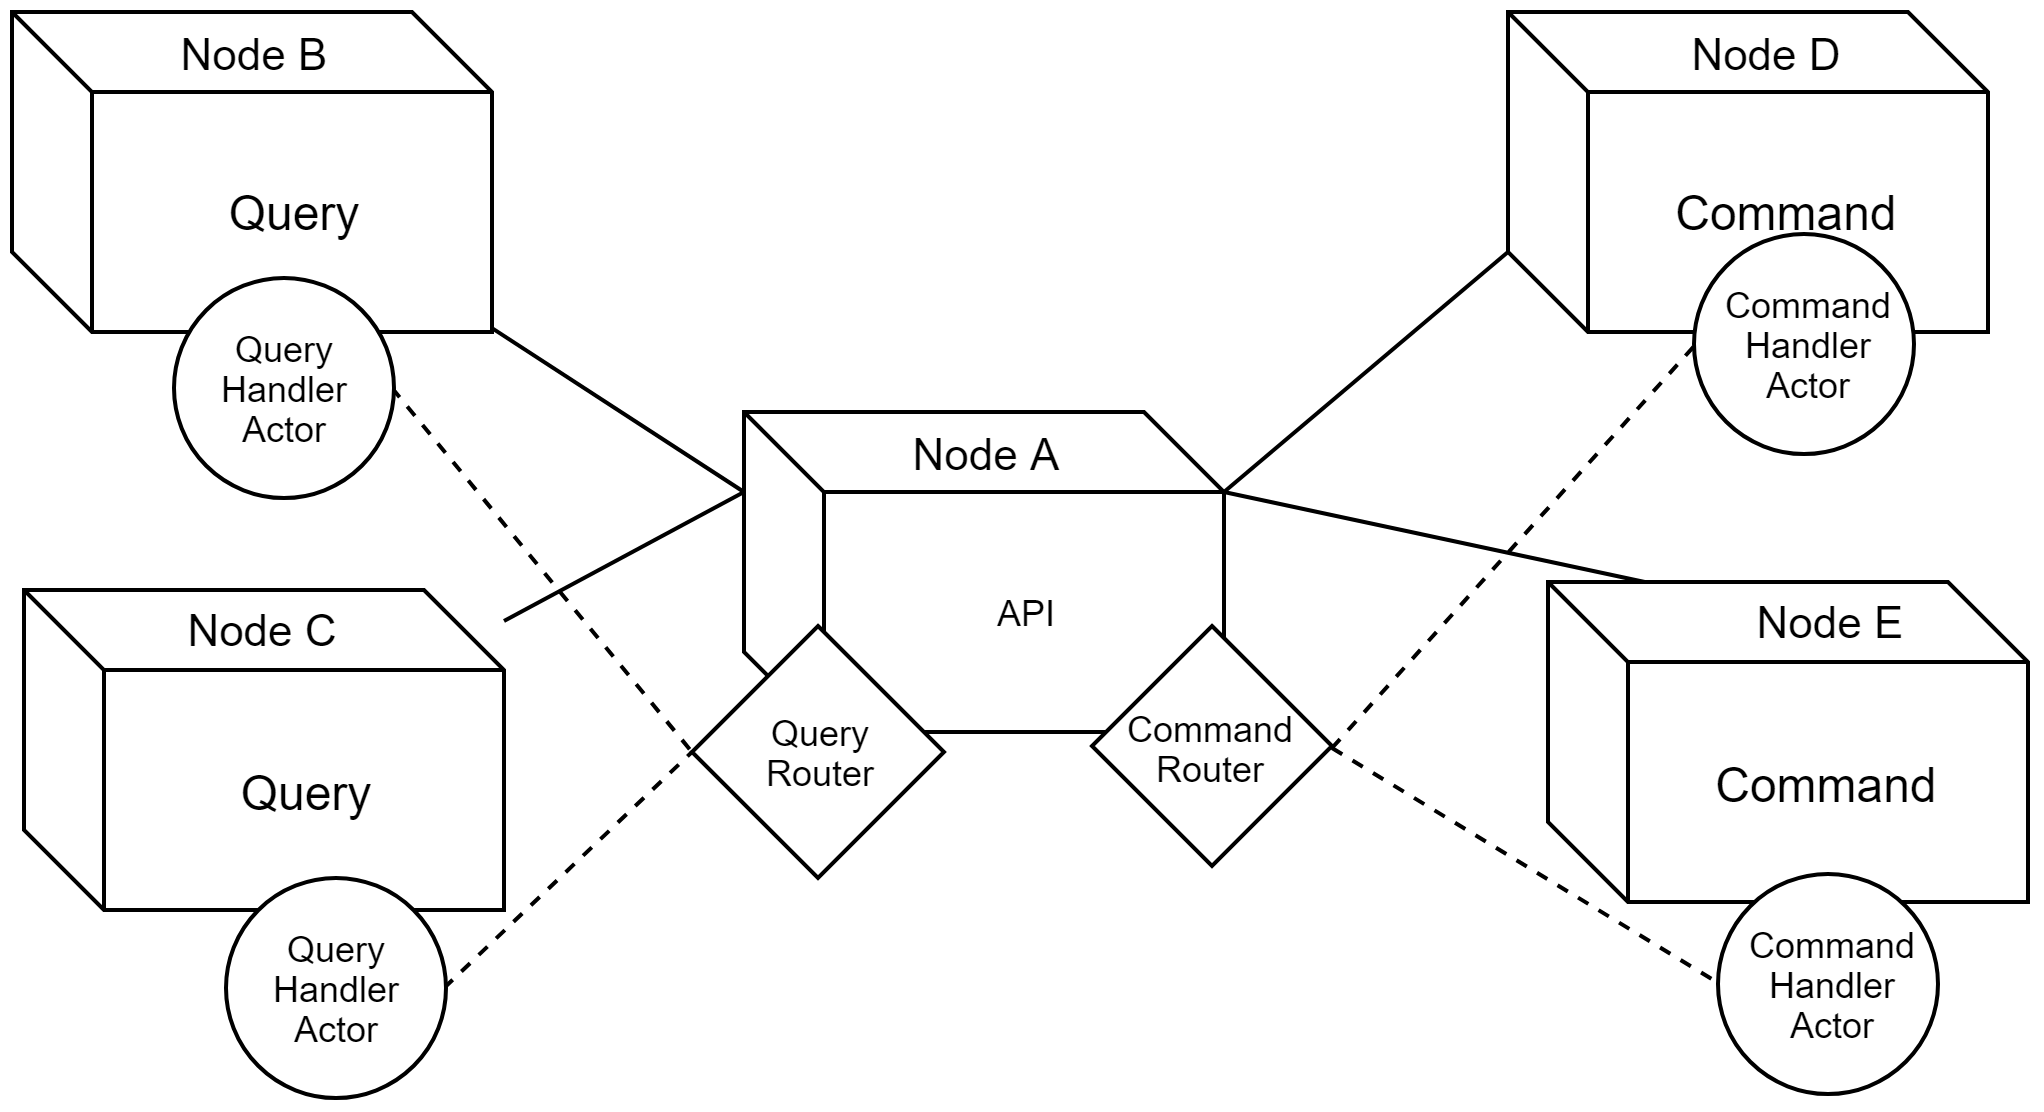
\includegraphics[width=\linewidth]{gfx/implementation/ClusterRouter}
  \caption{Ein \textit{Round-Robin} Router, welcher Nachrichten von der Komponente \textit{API} auf andere Komponenten verteilt.}
  \label{fig:implementation:routing}
\end{figure} 

\subsection{Gossip}
\label{subsec:implementation:gossip}
Bereits in Abschnitt \ref{subsec:implementation:lighthouse} wurde die Komponente \textit{Lighthouse} vorgestellt, welche als Einstiegspunkt für alle teilnehmenden Nodes verwendet wird. Die Verbindung zu den restlichen, im Cluster vorhandenen Nodes wird über das \textit{Gossip}-Protokoll hergestellt. \\
Gossip kommt aus dem Englischen, und beschreibt Klatsch-Gespräche innerhalb einer sozialen Gruppe. 
In dem Cluster-Protokoll Akka-\textit{Gossip} wird diese Art der Kommunikation angewendet, indem Nodes Änderungen am Clusterzustand ihren Nachbarn mitteilen \citep{Akka.netCommunityAkka.NETDocumentation}. \\
Nodes mit der Rolle \textit{Lighthouse} sind der Start dieser Kommunikation. Deshalb müssen diese Nodes auch über eine fixe Adresse verfügen, im Fall von \textit{TyrolSky} sind das Ip-Adresse sowie Port. Komponenten welche nun dem Cluster beitreten wollen, melden sich bei einem der \textit{Lighthouse}-Komponenten an und geben bekannt, über welche Adresse sie erreichbar sind. Über das \textit{Gossip}-Protokoll wird nun jedem bereits im System beigetretenen Node mitgeteilt, dass sich ein neuer Node im Cluster befindet. \\
In der Kommunikation zwischen den Nodes wird jedem einzelnen mitgeteilt, welche Rollen eine teilnehmende Instanz besitzt. Dies wird dann anschließend von den Routern, siehe Abschnitt \ref{fig:implementation:routing}, verwendet, um Nachrichten an diese Rolle zuzustellen. Das Protokoll beinhaltet auch Informationen über den aktuellen Zustand der einzelnen Nodes. So werden beispielsweise alle Nodes über eine fehlerhafte Verbindung zwischen zwei einzelnen Nodes benachrichtigt. Ist ein Node nicht mehr erreichbar, ohne dass eine kontrollierte Abmeldung vom Cluster stattgefunden hat, kann er nicht einfach aus dem Cluster entfernt werden. Um den fehlerhaften Zustand des Clusters zu lösen, soll eine Lösungsstrategie implementiert werden, welche wieder einen fehlerfreien Zustand herstellt, siehe dazu den nachfolgenden Abschnitt \ref{subsec:implementation:splitBrain}. \\ 
Das \textit{Gossip}-Protokoll dient, neben der Zusammenfügung der einzelnen Node zu einem Cluster, auch zum Austausch von Informationen über den aktuellen Zustand der einzelnen Nodes. Muss vom Protokoll eine Entscheidung getroffen werden, wie beispielsweise die Entscheidung, ob ein neuer Node dem Cluster beitreten darf, wird ein dafür definierter Node benötigt, welcher diese Entscheidungen treffen kann. Im Fall von \textit{TyrolSky} ist das immer der ältester Node im Cluster. Wird dieser vom Cluster entfernt, übernimmt die Führung der nächst älteste im Cluster enthaltende Node. Über diesen, in \textit{Akka.net} bezeichneten \textit{Leader}, werden Entscheidungen getroffen, welche für \textit{Gossip} relevant sind \citep{akkaInAction}. 

\subsection{Split-Brain} 
\label{subsec:implementation:splitBrain}
Wie bereits in Kapitel \ref{sec:distributedSystems:capTheorem} besprochen, kann bei einer Verbindung zwischen zwei Geräten jederzeit ein Problem auftreten, das die Kommunikation zwischen den Teilnehmern stört oder gänzlich unterbricht. Bei einer solchen Störung ist es dem betroffenen Node nicht mehr möglich, am \textit{Gossip} teilzunehmen und seinen Zustand anderen mitzuteilen. Auch wissen anderen Cluster Teilnehmer den Grund für Trennung der Kommunikation nicht. Deshalb können diese keine Aussage treffen, ob die Trennung des Teilnehmers nur temporär ist oder ob der Partner gar nicht mehr existiert. \\
Ein ähnliches Szenario kann auch auftreten, wenn zwei oder mehr Gruppen von Nodes zwar untereinander eine aufrechte Kommunikation führen, jedoch die Gruppen selbst voneinander getrennt wurden. So agiert jede Gruppe des Clusters für sich selber und kann sich mit den anderen Gruppen nicht mehr verständigen. Würde nun jeder Node im Cluster andere Nodes, welche für ihn nicht erreichbar sind, selbstständig entfernen, so würde jede Gruppe einen eigenen, neuen Cluster bilden, was als \textit{Split-Brain} bezeichnet wird \citep{networkIsReliable}. Bildet sich aus einem Cluster, durch gegenseitiges Entfernen, mehrere neue Clusters, so entstehen dadurch zwei oder mehrere Parallelstrukturen, welche die Konsistenz der gesamten Applikation verletzen können. Unter anderem werden die Prinzipien von \textit{Cluster Singletons} oder \textit{Sharding} verletzt und dies kann entsprechend zu Redundanzen führen. \\
In \textit{Akka.net} gibt es einige Strategieren, welche für das \textit{Split-Brain} Problem angewandt wurden. Jede Strategie hat jedoch einen Nachteil der teilweise sogar zum Stillstand der gesamten Anwendung führen kann. Nachfolgend die, laut \cite{Akka.netCommunityAkka.NETDocumentation} bereits verfügbaren, Strategien mit ihren Vor- und Nachteilen die durch dasFramework zur Verfügung stehen.
\begin{itemize}
  \litem{Statische Mehrheit}
  Jedem teilnehmenden Node wird die gleiche statische Nummer beim Start übergeben. Kann ein Node weniger Teilnehmer erreichen als die Nummer angibt, so beendet sich der Node selbstständig. Dadurch werden kleine gesplittete Gruppen automatisch beendet. Teilt sich jedoch das Netzwerk in mehr als zwei Gruppen auf, werden alle Nodes im gesamten Netzwerk beendet. 
  \litem{Behalte Mehrheit}
  Wird der Cluster durch ein Netzwerkproblem geteilt, wird anhand der zuletzt verfügbaren Informationen über den gesamten Cluster analysiert, ob der nun erreichbare Teil des Clusters die Mehrheit der vor der Unterbrechung beteiligten Nodes erreichen kann. Entspricht der neue Cluster der Mehrheit, werden die Nodes aufrechterhalten, anderenfalls werden alle Nodes des gesplitteten Clusters beendet. Auch hier kann das Aufteilen des Clusters in mehr als zwei Gruppen zum Stillstand des gesamten Clusters führen.
  \litem{Behalte Älteste}
  Durch das \textit{Gossip Protokoll}, siehe Abschnitt \ref{subsec:implementation:gossip}, wird mitgeteilt, zu welchem Zeitpunkt ein Node dem Cluster beigetreten ist. Darauf basierend kann berechnet werden, welcher Node der älteste im Cluster ist. Sobald sich der Cluster aufteilt, werden alle Nodes beendet, die den ältesten Node nicht erreichen können. Dadurch ist sichergestellt, das auch bei einer mehrfachen Aufteilung nicht der ganze Cluster beendet wird. Wird der Teil vom Node getrennt, der den ältesten Nodes und einige wenige andere Cluster beinhalteten, wird der gesamte größere Teil des Clusters beendet. Die Anwendung ist zwar nicht beendet, jedoch wurden mehr Nodes beendet als nötig. 
  \litem{Behalte Referenz}  
  Es wird ein fixer Nodes bestimmt, der für jeden Node erreichbar sein muss. Wird dieser von einem einzelnen nicht mehr erreicht, so wird dieser automatisch beendet. Dies führt dazu, dass wenn der referenzierte Node im gesamten Cluster nicht mehr erreichbar ist, die gesamte Anwendung beendet wird. Jedoch ist eine Aufteilung in zwei Teilen, der sogenannte \textit{Split-Brain} nicht möglich.
\end{itemize}
Für die Implementierung der \textit{TyrolSky} Anwendung wurde die Strategie \textit{Behalte Älteste} gewählt. Eine Zersplitterung des Clusters ist somit äußerst unwahrscheinlich. Das Risiko zu viele Nodes im Fehlerzustand zu beenden und das System somit kurzfristig zu verlangsamen, wird eingegangen, um die Datenkonsistenz für das \textit{Sharding} nicht zu verletzen.  

\subsection{Globale Dienste}
\label{subsec:implementation:singeltons}
Bereits in Abschnitt \ref{subsubsub:implementation:queryActorModel:resultPreparator} wurde ein Actor benötigt der nur exakt einmal im gesamten Cluster instanziiert werden darf um korrekt zu funktionieren. Im konkreten Beispiel war dies erforderlich, da der Actor für andere Actoren eindeutige, wiederverwendbare Namen generieren muss. In \textit{Akka.net} werden solche Actoren als \textit{Singletons} bezeichnet. Das Framework gewährleistet, dass die Actors die als Singletons deklariert sind, nur einmal im Cluster vorhanden sein können. Dabei wird auch berücksichtigt, dass wenn der Node auf welchem der Singleton Actor läuft, vom Cluster entfernt wird, der Singleton-Actor auf einen anderen Node im Cluster verschoben wird. Dadurch ist der Actor, mit Ausnahme der Zeit die der Prozess des Verschiebens von Actoren benötigt, zu jederzeit im System exakt einmal verfügbar. \\
Für die Überwachung und das Management der einzelnen Singleton-Actors ist der führende Cluster Node zuständig, siehe dazu Abschnitt \ref{subsec:implementation:gossip}. Jedem Singleton kann auch eine Cluster Rolle zugewissen werden, anschließend werden diese Singletons nur auf Nodes, welche dieser Rolle zugeordnet sind, ausgerollt. \\
Für die Implementierung von \textit{TyrolSky} wurden zwei Singletons eingesetzt. Beide werden für die Umsetzung der Namenverwaltung für die beiden Ergebnissaufbereiter im \textit{Query Service} benötigt. Den zwei Singletons wurde die Rolle \textit{Query} zugewiesen, womit sie nur auf den Nodes laufen, auf welchem sich die Ergebnisaufbereiter befinden.

\subsection{Verteilung transaktionaler Daten}
\label{subsec:implementation:akkaSharding}
Ein wesentlicher Teil der Komponente \textit{Domain Service}, Abschnitt \ref{subsec:implementation:domainService}, ist das Verteilen der Entitäten auf verschiedene Nodes der Rolle \textit{Domain Service}. Die Verteilung der Entitäten über den gesamten Cluster wird mit dem Prinzip des \textit{Shardings} umgesetzt. \\
Die Idee hinter \textit{Sharding} basiert auf Vorgehensweisen für verteilte Datenbanken und bedeutet laut \cite{shardingCattell}, dass Daten mithilfe eines Schlüssels auf unterschiedliche Hosts verteilt werden. Dabei bekommt jeder beteiligte Host einen bestimmten Bereich der Schlüsselmenge zugeteilt.
Die Information welche Schlüsselbereiche welchem Host zugeordnet sind, wird von jedem einzelnen Host geführt. Dadurch kann der Host durch den Schlüssel selber feststellen wo sich die entsprechende Datei befindet.
Dadurch ist eine effektive Verteilung von Daten auf unterschiedliche Hosts möglich, ohne das dabei jeder Beteiligte sämtliche Daten besitzen muss. Jedoch soll für eine Abfrage immer der dazugehörige Schlüssel bekannt sein. \\
Die Implementierung von \textit{TyrolSky} benützt diese Technik, mithilfe von \textit{Akka.net}, um Actoren über mehrere Nodes zu verteilen und dabei sicherstellen, dass diese von jedem anderen Node erreicht werden können. Dazu werden die Entitäten, also die Actoren welche im Sharding Cluster leben sollen, in \textit{Shards} unterteilt. Auf jedem Node der \textit{Shards} übernehmen soll, wird ein oder mehrere \textit{Shard Regions} gestartet. Dieser übernimmt, wie in Abbildung \ref{fig:implementation:actorSharding} dargestellt, die im zugewiesenen \textit{Shards} und startet die darin befindlichen Entitäten. Die Anzahl an möglichen \text{Shards} wird darbei für eine Anwendung fixiert. Im Falle von \textit{TyrolSky} werden {100} \textit{Shards} verwendet. Diese werden gleichmäßig an die verfügbaren \textit{Shard Regions} verteilt. Wird eine neue Region hinzugefügt, erfolgt eine Umverteilung der \textit{Shards}, womit auch die darin befindlichen Actors umverteilt werden. 

\begin{figure}
  \centering
  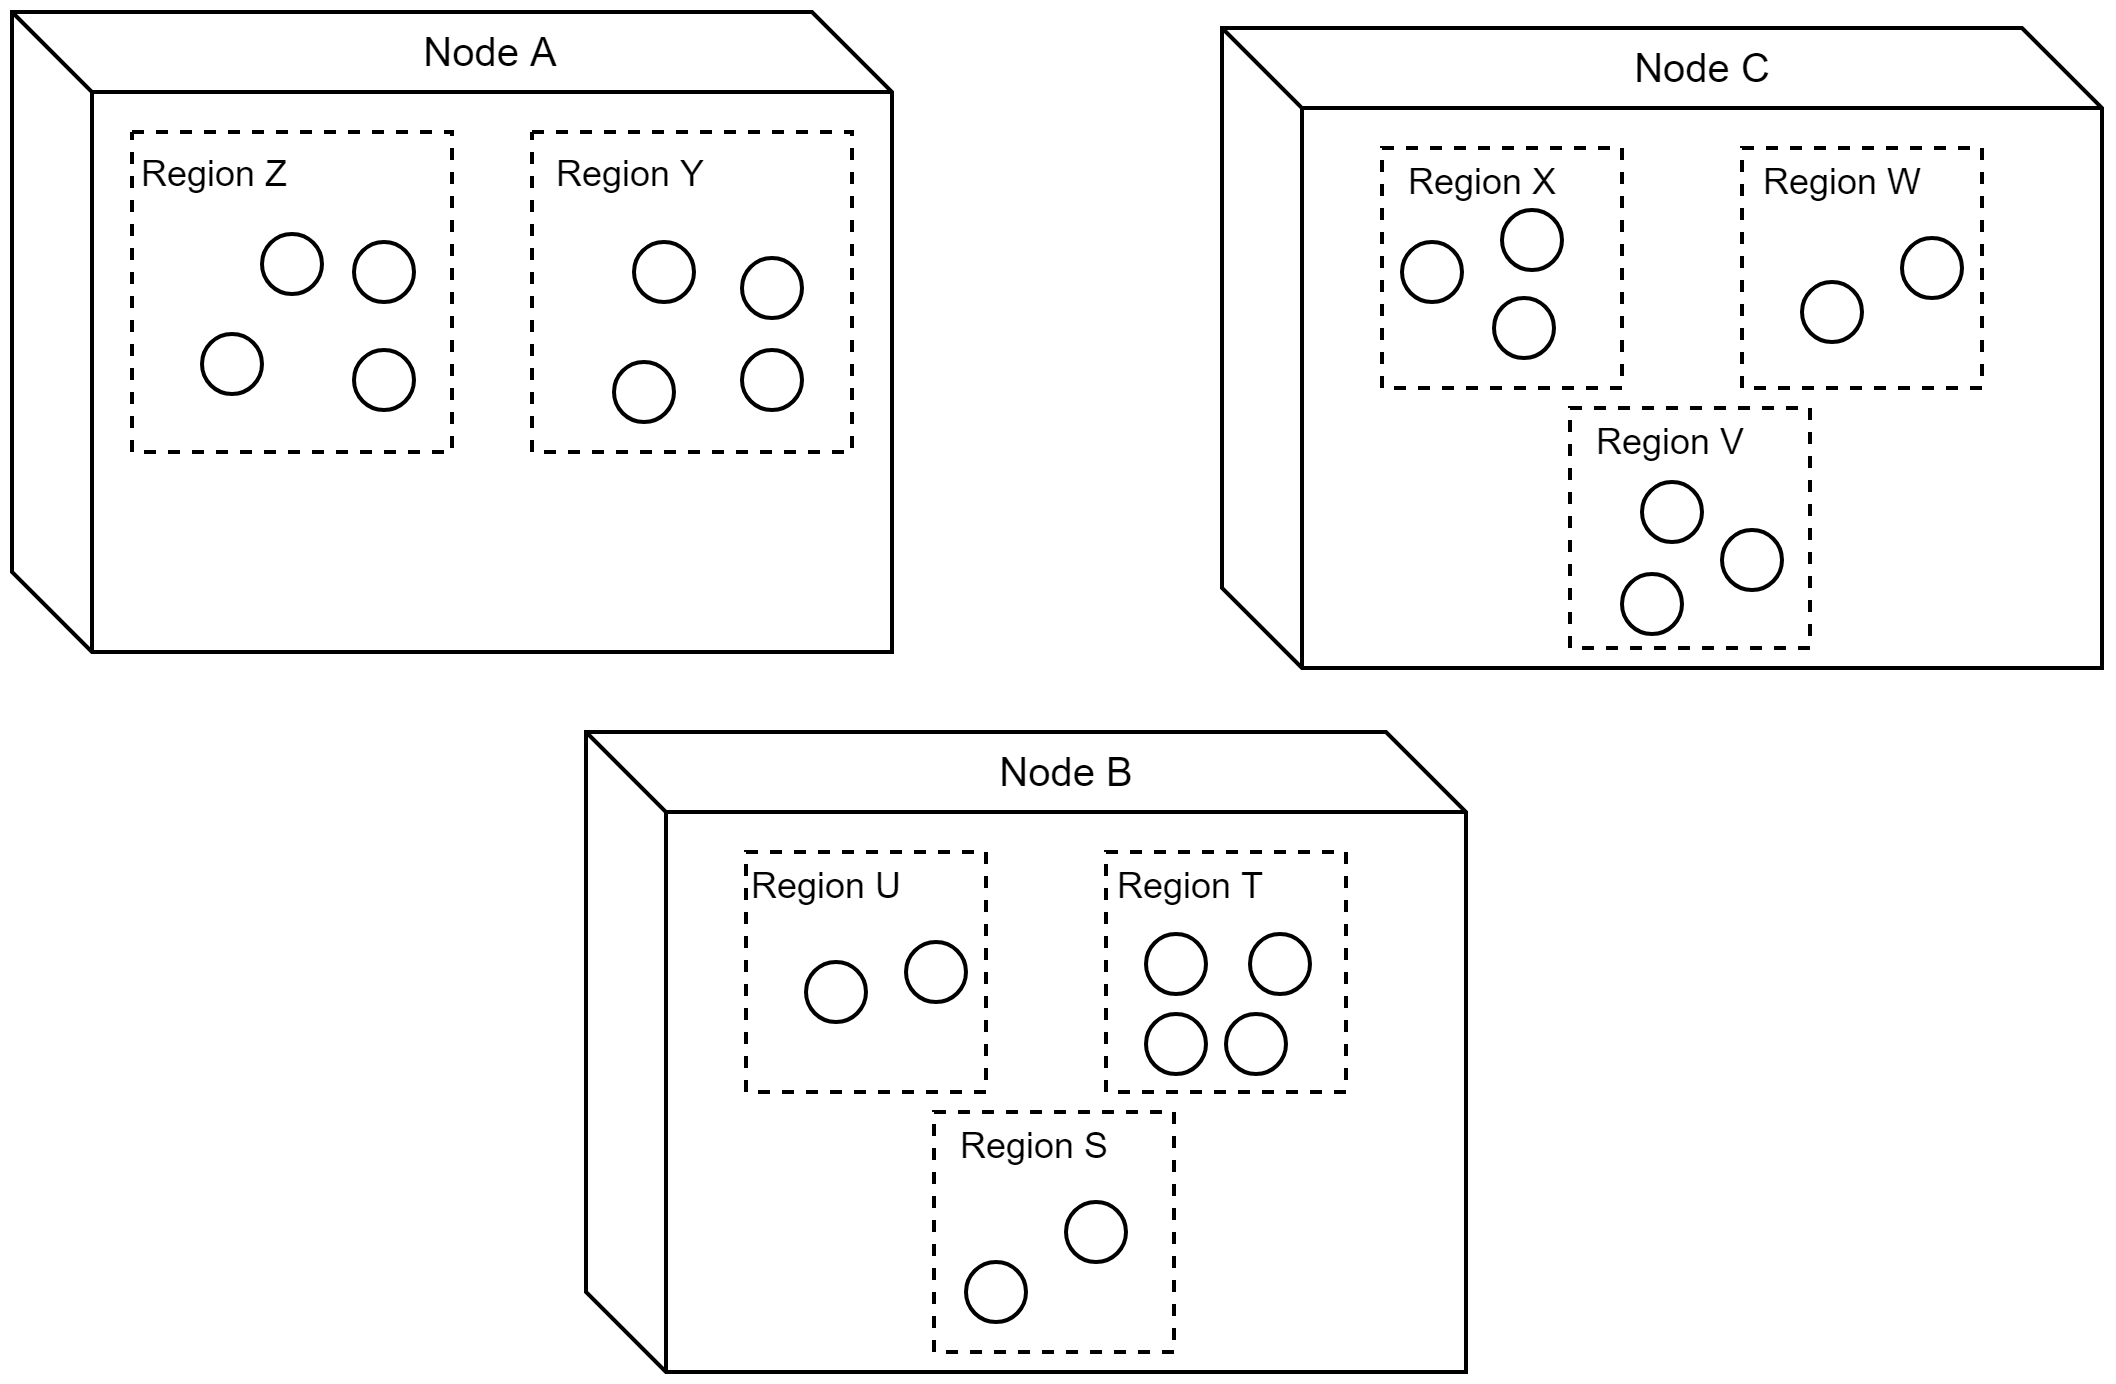
\includegraphics[width=0.8\linewidth]{gfx/implementation/Sharding}
  \caption{Verteilung von Entitäten in Shards, welche selbst wieder in \textit{Shard Groups} organisiert sind. Die Gruppen können zwischen den Nodes verteilt werden. }
  \label{fig:implementation:actorSharding}
\end{figure} 

Ein Grundprinzip von \textit{Sharding} ist die Unterteilung von Entitäten in unterschiedliche Gruppen, sogenannte \textit{Shards}. Dies wird in der \textit{Akka.net} Cluster Implementierung über die Zustellung von Nachrichten gelöst. Dazu werden Nachrichten nicht, wie bei Actor-Systemen, direkt an den Actor gesendet, sondern zuerst an einen Sharding Manager. Diese Nachrichten enthalten eine Identifikationsnummer der Entität, an die sie gerichtet sind. Der Manager interpretiert diese Nachricht und errechnet sich aus der Identifikationsnummer eine \textit{Shard} Identifikation. Anschließend prüft er, in welchem \textit{Shard Group} sich der \textit{Shard} befindet und welcher Node für diese Gruppe verantwortlich ist. Anschließend sendet er die Nachricht an den \textit{Shard Manager} auf dem entsprechenden Node. Hat sich dazwischen der \textit{Shard} auf einen anderen Node verschoben, kann der Node die Prüfung erneut durchführen und die Nachrichten an den neuen Zielort weiterleiten. Ist die gewünschte Entität am Node enthalten, stellt der dortige \textit{Shard Manger} die Nachricht an den entsprechenden Actor zu. \\
Für die Berechnung der \textit{Shard}-Identifikation auf Basis der Entitäts-Identifikation, wird in der Implementierung auf eine Hashfunktion zurückgegriffen. Der \textit{Shard Manager}, welcher die Nachricht an die zuständige \textit{Shard Region} weiterleiten soll, berechnet einen Integer Hashwert von der Entitäts-Identifikation. Diesen Wert Modulo der Anzahl an möglichen \textit{Shard Regions}, ergibt den \textit{Shard}, welcher für diese Entität zuständig ist. Die Anzahl der möglichen \textit{Shards} darf sich demnach zur Laufzeit des gesamten Clusters nicht verändern. Ansonsten würde durch die beschriebene Berechnungsfunktion neue \textit{Shards} entstehen und die Verteilung der Nachrichten schlägt fehlt. \\
Die Erzeugung von neuen Actoren in einem Shard wird durch Nachrichten an die noch nicht vorhandenen Actoren gestartet. Erhält ein \textit{Shard Manager} eine Nachricht an eine Entität, welche einem seiner \textit{Shards} zugeordnet werden kann und ist diese Entität noch nicht gestartet, so instanziiert der \textit{Shard Manager} einen neuen Actor. Dieser bekommt nun die Entitäts-Identifikation von der Nachricht zugewiesen.


\section{Garantierte Nachrichtenübermittelung}
Die gesamte Kommunikation zwischen Actors baut auf Nachrichten zwischen den beteiligten Actors auf. Wie bereits in Abschnitt \ref{sec:actor:patterns:guaranteedDelivery} diskutiert. kann die Zustellung einer Nachricht nicht, ohne verhältnismäßig viel Aufwand, garantiert werden. Wird in der \textit{TyrolSky} Anwendung eine Nachricht zwischen zwei Actors ausgetauscht wird die Nachricht höchstens einmal zugestellt. Das bedeutet das eine Nachricht unter bestimmten Umständen, wie beispielsweise Netzwerkfehler, nicht zugestellt wird und dies der Versender ohne spezielle Erkennungsmuster nicht mitbekommt. \\
Das Anwendungsumfeld von \textit{TyrolSky} benötigt jedoch auch Kommunikation, wo sichergestellt wird, dass die Zustellung einer Nachricht tatsächlich bis zum Empfänger funktioniert. Dies ist unter anderem der Fall, wenn ein Ticket sich selber storniert. Dabei muss sichergestellt sein, dass die zugehörige Passagierliste über die stornierung Informiert wird, um anschließend den dazugehörigen Sitzplatz für andere wieder freizugegeben. Dafür wurde die Garantierte Nachrichtenzustellung implementiert. Diese Zustellvariante ist eine Implementierung von garantierte \textit{Zustellung mindestens einmal}. \\
Die Ausführung der Garantierten Nachrichtenzustellung basiert auf Implementierung von \textit{Event-Sourcing}, beschrieben unter \ref{sec:implementation:eventSouring}. Dabei wird anstelle der Nachrichtenübermittelung an einen Actor mit den Methoden \textit{Tell} oder \textit{Ask}, siehe Abschnitt \ref{subsec:implementation:akka:cluster}, ein Event beim Sender Actor erzeugt, welches die Zustellung einer Nachricht an einen Actor signalisiert. Nach der erfolgreichen Speicherung des Events mit dem Namen \textit{GuaranteedMessageSent}, wird die Nachricht in einer Wrapper Nachricht vom Typ \textit{GuranteedMessage} zum Empfänger zugstellt. Zusätzlich wird im \textit{State} des Senders abgespeichert, dass diese Nachricht versendet wurde und eine Bestätigung erwartet wird. Trifft innerhalb einer konfigurierbaren Zeit, im Falle von \textit{TyrolSky} sind dies 5 Sekunden, keine Bestätigung für diese Nachricht ein, so wird diese erneut an den Empfänger zugestellt. Durch die Implementierung über \textit{Event Sourcing} werden nicht bestätigte Nachrichten auch nach einem neustart des Actors wieder versandt. \\
Trifft eine Nachricht vom Typ \textit{GuaranteedMessage} ein und wird bearbeitet, so wird eine Bestätigungsnachricht vom Typ \textit{Confirm}, welcher auch Informationen über die Orginal Nachricht enthält, an den Sender der ursprünglichen Nachricht gesendet. Empfängt dieser nun die Nachricht vom Typ \textit{Confirm} so markiert er die Original Nachricht als bestätigt. Somit kann der Sender Bestätigen das die Nachricht an seinem Zielort angekommen ist. Ist eine Zustellung nach mehreren Versuchen trotzdem nicht möglich, kann der Sender der Nachricht entsprechend darauf reagieren, hierfür ist jedoch eine angepasst Implementierung je nach Anwendungsfall notwendig. \\

\section{Externe Schnittstelle}
\label{sec:implementation:externalApi}
Neben der Interaktion mit Benutzern der \textit{TyrolSky}-Anwendung über die \textit{API}-Komponente, wird auch eine Kommunikation mit einem Fremdsystem benötigt. Um Abbuchungen an einem Konto vorzunehmen, wird, wie im Anforderungskatalog unter Abschnitt \ref{sec:Eruierung:technicalRequierements} gefordert, eine externe Anwendung angebunden. Diese Bankenanwendung operiert als eigenständige Anwendung und simuliert eine Bankenschnittstelle um Kontoabbuchungen von Kunden vorzunehmen. Die Simulationsanwendung selbst ist im nachfolgenden Kapitel \ref{subsec:implementation:bankApi} genauer beschrieben. \\
Der bereits in Abschnitt \ref{subsub:implementation:ChargingCoordinator}  beschriebene Buchungskoordinator verteilt Abbuchungstransaktionen, mithilfe von \textit{Sharding}, innerhalb des Clusters auf verschiedene Nodes. Jede Transaktion benötigt jedoch eine Kommunikation mit der Bankenschnittstelle, um die Transaktion durchzuführen und sie mit dem Bankensystem abzugleichen.  \\
Dazu wird auf jedem Node der Buchungen durchführen kann, das sind alle Nodes mit der Rolle \textit{Domain-Service}, ein \textit{BankingActors} Actor gestartet. Dieser ist anschließend für die Kommunikation mit der Bankenanwendung zuständig. \\
Möchte nun eine Transaktion eine Kommunikation mit der Bankenanwendung starten, sendet diese einen Befehl in Form einer Nachricht an den \textit{Banking-Actor}. Der \textit{Banking-Actor} befindet sich auf dem gleichen Host wie der Transaktions-Actor. Der Befehl an den \textit{Banking-Actor} enthält Informationen über die gewünschte Kommunikation mit der Bankenschnittstelle. Wird während der Kommunikation zur Bank der betroffene Transaktions-Actor durch \textit{Sharding} verschoben, betrifft dies nicht den BankingActor selbst, da dieser fix auf jedem Host als eigene Actor Instanz vorhanden ist. 
\subsection{Banken API}
\label{subsec:implementation:bankApi}
Für die Anbindung einer externen Bank wurde eine eigene Software geschrieben, die eine simulierte und einfach gehaltene  Bankenschnittstelle zur Verfügung stellt. Die \textit{BankChargingAPI} ist komplett getrennt von der restlichen Implementierung der \textit{TyrolSky} Anwendung und kann über eine eigene \textit{REST}-Schnittstelle angesprochen werden. \\
Die Kernaufgabe dieser Bankensimulation ist es, Bankkonten zu verwalten. Dazu werden in einer relationalen Datenbank Kontoinformationen abgebildet. Dabei hat jedes Konto einen Namen sowie einen aktuellen Guthabenstatus. Für die Bankentransaktionen, nicht zu verwechseln mit den Transaktion innerhalb der \textit{TyrolSky}-Anwendung, wird eine eigene Tabelle geführt, welche Informationen über jede bearbeitete Transaktion enthält. Die Transaktion enthält Informationen über den eigenen Status sowie den Transaktionsbetrag. Über die Schnittstelle kann auch der Status einer Transaktion abgefragt werden. Diese Transaktionsstatus-Abfrage wird auch von der \textit{TyrolSky}-Anwendung verwendet um die eigene Flugbuchung zu kontrollieren, beschrieben unter Abschnitt \ref{subsub:implementation:ChargingCoordinator}. \\
Für die Implementierung der Simulationsanwendung wurde auf eine \textit{SQL-Datenbank} zurückgegriffen. Jeder Zugriff auf die Datenbank erfolgt in einer Transaktion mit dem strengen Transaktionslevel \textit{Serializable}, wodurch keine Inkonsistenzen der Kontoinformationen entstehen können \citep{adya2000generalized}. Durch die Transaktionstabelle ist eine Nachvollziehbarkeit der getätigten Transaktionen möglich. \\
Die Simulationsanwendung \textit{BankChargingAPI} bietet folgende Schnittstellen für die \textit{TyrolSky}-Anwendung an:
\begin{itemize}
    \litem{ChargeAccount}
        Mit Angabe des gewünschten Kontos sowie dem abzubuchenden Betrages wird eine Transaktion gestartet. Für den Aufruf wird eine Transaktionsnummer angegeben, mit der später der Status der Transaktion abgefragt werden kann.
    \litem{GetTransactionStatus}
        Durch Angabe der Transaktionsnummer wird der aktuelle Status der Transaktion zurückgegeben. 
\end{itemize}
Durch die Aufteilung in zwei Methoden ist es möglich im Fehlerfall Transaktionsinformationen nicht zu verlieren. Wird beim Aufruf der \textit{ChargeAccount} Schnittstelle kein Ergebnis zurückgeliefert, kann der Status über \textit{GetTransactionStatus} zu einem späteren Zeitpunkt abgefragt werden.

\section{Testapplikation}
\label{subsec:implementation:TestApplikation} 
Die \textit{TyrolSky}-Anwendung bietet eine Schnittstelle für Endbenutzer an, mit der die Anwendung bedient werden kann. Um eine größere Menge an Benutzern und somit Anfragen zu simulieren wird eine eigene Testapplikation benötigt. Diese bietet die Möglichkeit eine Vielzahl an Flügen zu reservieren sowie zu buchen. Für jede Anfrage an das \textit{TyrolSky}-System wird die Anfrage protokolliert und der Rückgabewert der Anfrage abgespeichert. Dadurch können nach einem Testdurchlauf die Resultate eingesehen und mit dem Zustand des getesteten Systems verglichen werden. \\
Die Umsetzung der Testapplikation fordert einen hohen Grad an Parallelisierung, da gleichzeitig eine Vielzahl an Anfragen an das System gestellt werden sollen. Aufgrund der Anforderung an eine bestmögliche Parallelisierung wird die Anwendung mit dem Actor-Model, das für Parallelisierte Anwendungen konzipiert wurde, siehe dazu \ref{actor:parallelism}, realisiert. Wie die Implementierung der externen Bankenanwendung ist auch die Testapplikation eine vollständig eigenständige Anwendung, welche keinen Zusammenhang mit der Implementierung der \textit{TyrolSky}-Anwendung besitzt. \\
Jede Anfrage, die zum testenden System durchgeführt wird, ist in einer Datenbanktabelle protokolliert. Dabei werden Informationen zur Anfrage selbst, wie Flugnummer, Flugdatum und Passagierinformation sowie Informationen zur Buchungs selbst abgespeichert. Der genaue Aufbau der Tabelle \textit{StressTest}, welche alle Informationen über eine Anfrage enthält, ist aus Abbildung \ref{fig:implementation:stressTestDbSchema} zu entnehmen.
\begin{figure}
    \centering
    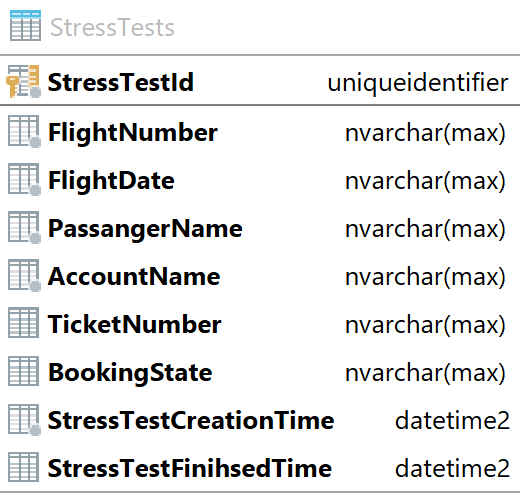
\includegraphics[width=0.4\linewidth]{gfx/implementation/stressTestDbSchema}
    \caption{Datenbankschema für die Testapplikation der \textit{TyrolSky}.}
    \label{fig:implementation:stressTestDbSchema}
\end{figure} 

Die Testanwendung wird in Form einer Konsolenanwendung ausgeführt. Dabei kann beim Start der Anwendung über Parameter angegeben werden, welche Flüge zu welchem Ausmaß gebucht werden sollen. Die Anwendung startet anschließend die entsprechenden Schritte, um Flüge zu buchen. 

\subsection{Ablauf eines Testes}
Nach dem Starten der Konsolenanwendung werden die übergebenen Parameter ausgelesen und das Actor-System für den Testlauf erzeugt. Anschließend wird die vom Tester geforderte Anzahl an Buchungen durchgeführt. Für jede Buchung wird ein eigener Buchungs-Prozess gestartet, welche in der Tabelle \textit{StressTest} abgebildet sind. Dabei wird zuerst versucht, ein Ticket zu reservieren. Konnte eine Reservierung erfolgreich durchgeführt werden, versucht die Anwendung diese Reservierung abschließend zu buchen.
Die für die Buchung benötigten Kontoinformationen werden  ebenfalls in der Tabelle \textit{StressTest} zur aktuell getesteten Buchung abgespeichert. Die Testanwendung fragt nach der Buchungsaufforderung, das zu testenden System nach dem Buchungsresultat, bis dieses einen endgültigen Buchungsstatus zurückliefert. \\
Die einzelnen Buchungsjobs werden dabei nicht alle gleichzeitig gestartet. Alle zwei Sekunden beginnen 10 neue Jobs, diese laufen jedoch parallel bis zur Fertigstellung des Jobs weiter. Die Gesamtanzahl an Jobs wird über die Parameter der Anwendung gesteuert. Ist die Testanwendung beendet, kann das Resultat in der Datenbank abgefragt werden. Weiters können durch die Angabe der Kontoinformationen die Resultate mit der \textit{BankChargingAPI}-Anwendung sowie mit den entsprechenden Passagierlisten der \textit{TyrolSky}-Anwendung verglichen werden.

\subsection{Parameter Beschreibung}
Für die Steuerung und Parametrisierung der \textit{TyrolSky} Testapplikation können folgende Parameter zum Starten der Konsolenanwendung angewandt werden:

\begin{itemize}
    \litem{NumberOfBookings} Gesamtanzahl der zu buchenden Tickets
    \litem{FlightsToBook} Angabe einer Liste an verschiedenen Flugnummern, die gebucht werden sollen
    \litem{DateRangeStart und  DateRangeStop} Start- und Enddatum für den Zeitraum, in der ein Flug stattfinden soll
    \litem{ChargingAccounts} Fiktive Bankkonto-Informationen, mit denen die Flüge bezahlt werden sollen
\end{itemize}
Die Testanwendung versucht anschließend die angegebene Anzahl an Tickets zu reservieren sowie zu buchen. Dabei wird für jedes Ticket zufällig ein Datum sowie eine zufällige Flugnummer ausgewählt. 


\section{Verwendete Umgebung}
Für die Umsetzung sowie den Betrieb der \textit{TyrolSky} Anwendung wurden unterschiedliche Fremdkomponenten eingesetzt. Die Tabelle \ref{tab:implementation:EnvironmentVersions} gibt einen Überblick über die maßgeblich eingesetzten Komponenten sowie Softwaresystemen. 

\begin{table}[h]
    \centering
    \begin{tabular}{llp{6.5cm}}
    Name            & Version       & Beschreibung \\ \hline
    C\#          & 7.0               &  Programmiersprache mit welcher alle Teile der Anwendung umgesetzt wurden. \\
    DotNetCore      & 2.0.0             &  Laufzeitumgebung der Entwickelten C\# Programme \\
    Akka.net        & 1.3.5             & Framework für die Umsetzung des Actor Models mit C\# \\
    Akka.net Sharding & 1.3.5-beta60    & Erweiterung für Akka.net um Sharding zu ermöglichen \\
    Akka.net Persistence Sql & 1.3.2    & Ermöglicht die Speicherung des Akka.net EventStores in einer SQL Datenbank\\
    SqlServer       & 2017 14.0.3025.34 & Datenbank Server für den EventStore sowie die Datenbank für die Testanwendung\\
    Docker          & 18.03.1           & Containerbasierte Infrastrukturumgebung für die benötigten verschiedenen Anwendungen\\
    \end{tabular}
    \caption{Die in \textit{TyrolSky} verwendeten Bibliotheken sowie die für den Testbetrieb verwendete Software}
    \label{tab:implementation:EnvironmentVersions}
    \end{table}